\chapter{Evaluation of Platforms} \label{chap:evaluation}
\section{General concepts}
Before going into comparison, the general concepts of the three platforms will be quickly recapped to provide a basis about the working mechanism of these platform. More detail elaboration of their features will be presented during the evaluation.

\textbf{Apache Kafka}

\begin{figure}[h]
	\centering
	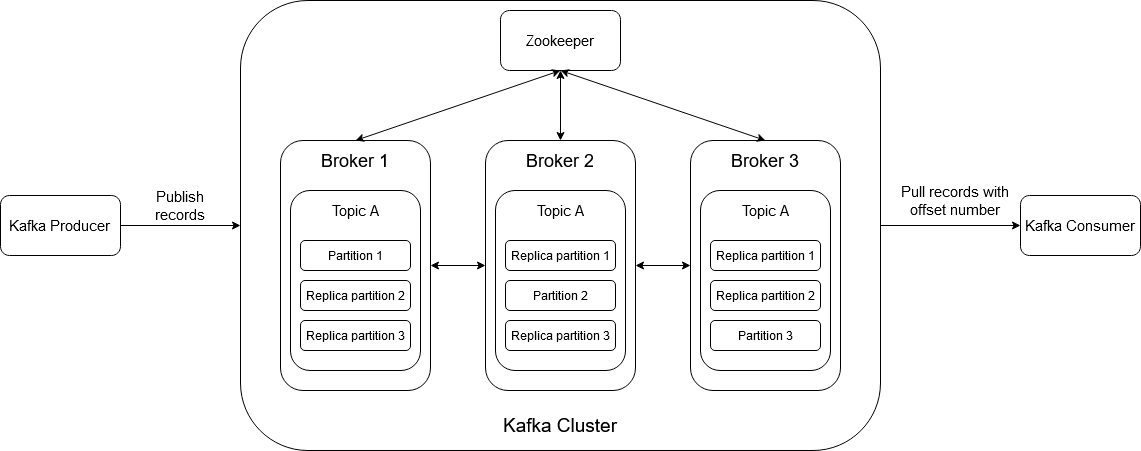
\includegraphics[width=12cm]{images/general-kafka.png}
	\caption{General concept of Apache Kafka.}
	\label{fig:kafkageneral}
\end{figure}


Apache Kafka is a platform designed specifically for event streaming. There are a number of fundamental concepts and core components of Kafka:
\begin{itemize}
	\item Record: this is the name for message published to Kafka. Each record can have a key, a value, and some metadata. This is also usually referred as event or message.
	\item Kafka broker: this is the heart of Kafka. A broker is in charge of serving read/write requests and persisting published messages from clients to its disk. Kafka usually runs in cluster with three or more broker. In the current release of Kafka, the cluster also include one or more Apache Zookeeper \cite{apachezookeeper} nodes to maintain metadata of these brokers. However, Zookeeper will soon be removed completely from Kafka in later release and metadata will be maintained natively on Kafka broker instead \cite{kafkaremovezookeeper}.
	\item Topic and partition: Records are organized into different topics on Kafka. A topic further comprises of multiple partitions, each of which is an append-only and immutable log. New records will be appended to the end of the log. Each record in a partition is uniquely identified by an incremental offset number. There are two types of partition, namely, leader and follower. Read and write operations will be done on the active leader partition. Follower partitions are replicas of the leader which reside on different brokers in the cluster and cannot serve requests. Since Kafka 2.4, it is possible to read records from follower replicas as well \cite{kafkareadfromfollower}. Nevertheless this feature is disabled by default.
	\item Kafka clients: There is Producer \acrshort{api} which is used to publish records to Kafka topics. On the other hand, Consumer API is used to read records from a Kafka topic. 
\end{itemize}

In this thesis, the current release 2.6.0 of Kafka will be evaluated.

\textbf{Apache Pulsar}

\begin{figure}[h]
	\centering
	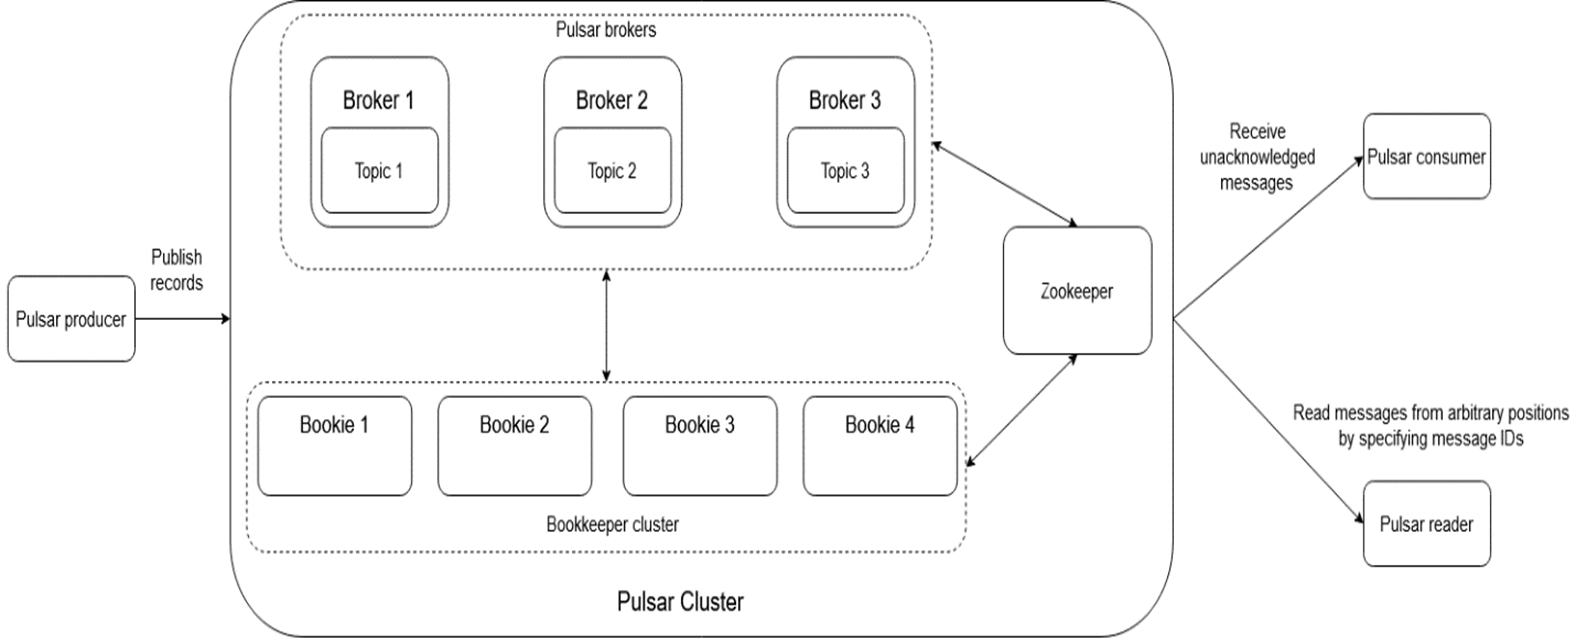
\includegraphics[width=12cm]{images/general-pulsar.png}
	\caption{General concept of Apache Pulsar.}
	\label{fig:pulsargeneral}
\end{figure}

Apache Pulsar is designed as a multiple-purposed platform by combining the concept of traditional messaging and event streaming. Following are the main concepts of Pulsar:
\begin{itemize}
	\item Message: a message published to Pulsar has a key-value format along with some metadata.
	\item Pulsar broker: this component is responsible for serving read/write requests from clients and send persisting request of messages to the persistence layer. There are usually many brokers run together in a cluster.
	\item Apache Bookkeeper \cite{apachebookkeeper}: this is the persistence layer of Pulsar. Bookkeeper handles the durable storage of messages upon receiving requests from the Pulsar broker. Messages are stored on Bookkeeper ledgers which are immutable logs with new records being appended to the end. The Bookkeeper usually runs in a cluster with multiple nodes which are called Bookies. 
	\item A Pulsar cluster is made from a cluster of Pulsar brokers, a cluster of Bookkeeper nodes and also a number of Zookeeper nodes for metadata management of these clusters.
	\item Topic and partition: Apache Pulsar organize records into different topics. Each broker is responsible for read/write request of a different subset of topics. A topic can also be split further into multiple partitions. However, a partition is internally also a normal Pulsar topic which is managed transparently to user by Pulsar. Records in a Pulsar partition or a non-partitioned topic are uniquely identified by message IDs.
	\item Pulsar clients: Messages can be published to Pulsar topic with Pulsar Producer API. For messages consumption, there are two different client APIs, namely, Consumer API and Reader API. Each of these consumption clients has different level of flexibility and can be used in different cases. The detail comparison of Consumer and Reader is given in the evaluation section of messaging patterns.
\end{itemize}

The current release 2.7.0 of Pulsar will be evaluated.

\textbf{NATS Streaming}
\begin{figure}[h]
	\centering
	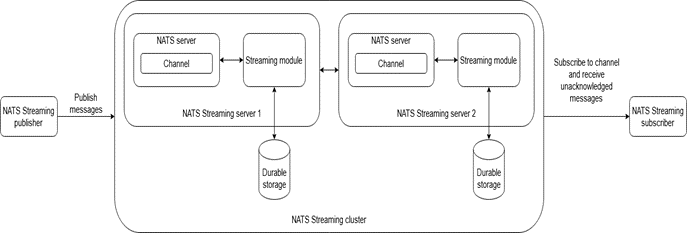
\includegraphics[width=12cm]{images/general-nats.png}
	\caption{General concept of NATS Streaming.}
	\label{fig:natsgeneral}
\end{figure}

NATS Streaming is an event streaming add-on built on top of NATS server which is a messaging system without persistent layer. It has some core concepts:
\begin{itemize}
	\item Message: a message published to NATS Streaming contains a value and some metadata.	
	\item NATS Streaming server: A NATS Streaming server comprises of a normal NATS server as the messaging layer and a a separated streaming module which is internally a normal NATS client to receive and persist message on NATS server to a pluggable durable storage.  Because of this special structure, the clients and streaming module only interacts indirectly via the intermediate NATS Server and all requests must first traverse through the NATS Server. NATS Streaming comes with an embedded NATS server but can also be configured to work with an existing NATS server. A number of NATS Streaming servers can be grouped together into a cluster in two modes: clustering and fault tolerance. In the first mode, each server retains a full copy of all messages in a separated data store. In the latter mode, nodes in the cluster share a single data store.
	\item Channel: On NATS Streaming, messages are organized into channels which internally are made from append-only message logs. A message in a channel can uniquely be identified with an incremental sequence number.
	\item NATS Streaming client: NATS streaming provides client API to publish and subscribe to messages on channels.  
\end{itemize}
In the thesis, the latest version 0.19.0 of NATS Streaming is used for assessment.

Moreover, each platform provides different implementations of its clients in different programming languages. Nevertheless, to have a uniform benchmark, when the evaluation involves comparing clients, the Java implementations will be used since this programming language is officially supported by all three platforms.

\section{Event storage} \label{section:eventstorage}
\large \textbf{Apache Kafka}\\
\normalsize
\textbf{Durable storage}

In Kafka, records are stored in partitions each of which is stored on the disk as a number of segment files \cite{kafkaimplementation}. The broker receives records and writes them sequentially to these files. When a segment file reaches its configurable maximum size, a new file will be created for writing new records. Since all records are only appended to these files, the read/write of records only requires sequential I/O on the disk. This is one of the key design features of Kafka to help maintain fast performance even on cheap hard disks.  

However, a Kafka broker can already acknowledge writing requests when records are written to I/O buffer and not necessarily when records are persisted to disk. Therefore, durability is not guaranteed, and message loss can still happen when the broker fails before flushing records to disk. User can force disk flush to ensure durability whenever a message is received but this is not recommended by Kafka since it can reduce the throughput of the system \cite{kafkaconfigurationtopic}. To achieve durability, a more common approach is combining this unflushed write feature with redundant write on other brokers in the cluster which is the fault-tolerance feature for storage provided by Kafka. This is elaborated in more detail in the next section.

\textbf{Event storage is fault tolerant}\\
As briefly mentioned in the general concept, there are two types of Kafka partitions, namely, leader and follower. The leader partition is active and can serve read/write requests from clients while followers are standby replicas of the leader. For fault tolerance, Kafka supports data replication among brokers in the cluster \cite{kafkadatareplication}. For each topic, user can specify a replication factor which determines the number of existing copies of records on Kafka.  When replication factor is 2 or more, every partition of the topic will have 1 leader and 1 or more followers. For each partition, each of its copies will be distributed on a different broker in the cluster. Therefore, there will be no single point of failure for record storage. The replication factor must be equal or smaller than the number of brokers in the Kafka cluster.

However, enabling only data replication on the broker cannot guarantee that all records are safely replicated on the Kafka cluster.  By default, a Kafka producer sends a record and only waits for the acknowledgement of successful write from the leader partition. If the broker with the leader partition goes down before the record is flushed to its disk and replicated to other follower replications, the record may be lost without the producer knowing about it for resending. Therefore, the producer must be strictly configured to wait for acknowledgements from the leader partition as well as other follower replicas. In this case, the leader partition will also wait for acknowledgements from its followers before confirming with client. By having the redundant acknowledgements, durability is guaranteed even when messages are not yet persisted to disks given that all brokers retaining the partition do not fail simultaneously. 
\begin{figure}[h]
	\centering
	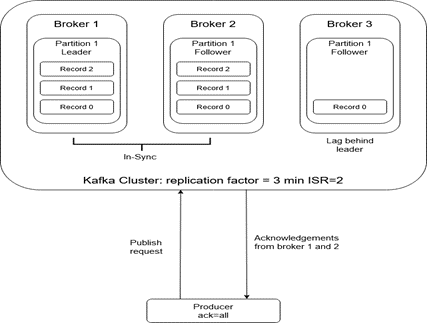
\includegraphics[width=12cm]{images/ft-eventstorage-kafka.png}
	\caption{Data replication model for fault tolerance of event storage on Kafka.}
	\label{fig:fteventstorekafka}
\end{figure}

For each replicated partition, the follower periodically fetch data from leader to stay in-sync. If the producer waits for acknowledgements from all replicas, some followers may fall too far behind the leader (e.g. due to slow network connection) and increase the waiting time of the producer. Therefore, the leader of the partition dynamically maintains a list of in-sync replicas (\acrshort{isr}) which contains itself and all followers which currently stay synchronized with it. This list is stored on Zookeeper. When a follower does not catch up with the leader by sending fetch request after a configured amount of time, it will be removed from the ISR of the partition. The slow follower can rejoin ISR later when it has fully caught up with the leader partition. In practice, the producer will only wait for acknowledgements from the ISR instead of all replicas. This aims at balancing between the durability, fault-tolerance of published records and the latency for acknowledgement. As a result, a message acknowledged to producer can survive up to \emph{ISR-1} failed nodes and still be available to consumer.

It could be possible that all followers of a partition are out-of-sync with the leader. In this case, producer only receives one acknowledgement from the leader which brings back the problem of losing messages. Therefore, Kafka also provides the option to configure the minimum number of in-sync replicas. If the ISR falls below this number, new writing requests will be rejected, and availability is compromised to ensure the durability.

Durability and fault tolerance of data storage on Kafka are closely related to each other and can only be achieved with the right configurations on both Kafka brokers and Kafka producers. In addition, Kafka provides many configuration options to give users the flexibility to choose different priorities for their systems such as availability, durability, latency. 

\textbf{Flexible data retention policy}\\
All records published to Kafka will be retained. Old data can be cleaned up with different cleanup policies \cite{kafkaconfigurationtopic}. These policies can be configured on the broker level which will then be applied to all topics or they can be configured differently for individual topic. There are two basic strategies to retain data:
\begin{itemize}
	\item Delete: All records are retained for a period of time or based on a maximum size and then they will be deleted.
	\item Compact: This strategy is only applicable to records with key values. The topic will be compacted. Only the latest record of each key value is retained.
\end{itemize}

For the first strategy, user can choose different retention policies for a partition based on maximum size of a segment file of a partition or based on retention period. Once the retention limit is exceeded, oldest segment file of the partition will be deleted. By default, there is no limit on the size of a partition and the retention period is 7 days. User can also configure infinite retention period if necessary.

\begin{figure}[h]
	\centering
	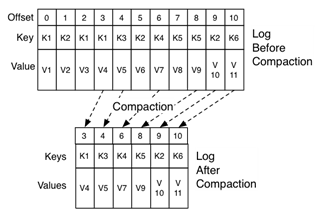
\includegraphics[width=10cm]{images/compact-kafka.png}
	\caption{Log compaction on Kafka (taken from Kafka documentation \cite{kafkadesignlogcompact}).}
	\label{fig:compactekafka}
\end{figure}
For the second strategy, the background cleaner thread of Kafka will regularly scan the segment files and keep only the latest record for each key value (figure \ref{fig:compactekafka}). Therefore, this only works with records with non-empty key value. Writing request of record without a key to a topic configured with compact cleanup policy will be rejected.


The two strategies can also be combined. With this setup, topics will be compacted regularly but when the retention maximum size or maximum retention period is reached, the data will also be removed regardless of being compacted or not. For example, in case of an online shopping application where each order is kept track by a sequence of events published to Kafka as records, when users are interested in the latest status of an order but only if the order is not older than 3 months, it is reasonable to use this combination of retention strategies.

To sum up, Kafka provides a flexible way to retain all records or only selective data. Users can choose the appropriate strategy based on their use cases. 

\large \textbf{Apache Pulsar}\\
\normalsize
\textbf{Durable storage}

A Pulsar topic can be persistent or non-persistent which must be specified by user when creating the topic. Messages on non-persistent topics are only kept in-memory on the Pulsar brokers. For persistent topics, Pulsar provides the persistence layer using Bookkeeper.  A Pulsar broker has a Bookkeeper client internally. When receiving writing requests from clients, Pulsar broker sends persistent requests to the Bookkeeper cluster. Bookkeeper provides the storage abstraction called ledger. A Pulsar topic is made up from one or more ledgers. New messages will be appended to the end of a ledger. Once a ledger reaches its maximum size or the Bookkeeper node (Bookie) is restarted, a new ledger will be created. Internally, a Bookie stores messages of a ledger in an entry log file on its disk. Durability of data on a Bookie is guaranteed once an acknowledgement is sent back to Pulsar broker. The broker then can confirm the successful write with client.

\textbf{Event storage is fault tolerant}\\
Pulsar supports replication of messages of a topic on multiple Bookies for fault-tolerance. To achieve this, Pulsar utilizes the built-in replication mechanism of Bookkeeper. A Pulsar topic comprises of one or more Bookkeeper ledgers. Each ledger can be further made from one or more fragments. When a ledger is created, it must have three important configuration options which control how messages are written and replicated on Bookkeeper cluster \cite{bookkeeperprotocol}:
\begin{itemize}
	\item Ensemble size (E): An ensemble is a set of Bookies which are selected randomly from the Bookkeeper cluster to persist records for a fragment of the ledger. Whenever one node in the ensemble fails to accept write requests, a new fragment with a different ensemble without the failed node is created for the ledger to ensure that there are enough available Bookies for writing. The ensemble size can be configured by user and must be equal or smaller than the number of nodes in the Bookkeeper cluster.
	\item Write quorum size (Qw): Every record in a fragment will be written to Qw nodes in the ensemble so that each record will have Qw copies for fault tolerance. Qw can be equal or smaller than E. If it is smaller than E, every record will be written to a different subset of nodes in the ensemble.
	\item Acknowledge quorum size (Qa): This number specify the number of nodes in the Qw set which must acknowledge before a message is considered to be successfully persisted. Write request is acknowledged by Pulsar broker when Qa Bookie nodes have confirmed receiving the message. This option provides a possibility to balance between performance and the persistence guarantee. With this configuration, it is guaranteed that a message can still survive and be available in case \emph{Qa – 1} Bookies are destroyed.
\end{itemize}

\begin{figure}[h]
	\centering
	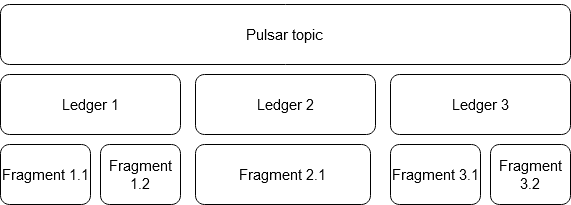
\includegraphics[width=12.5cm]{images/pulsar-topic.png}
	\caption{Underlying storage layers of a Pulsar topic.}
	\label{fig:pulsartopic}
\end{figure}
Although all these configuration options are from Bookkeeper which is used internally by Pulsar, Pulsar also allows users to configure them using its administrator tool to achieve the required level of fault tolerance in different use cases. When there are not enough Bookies to meet the configured ensemble size and quorum, writing request from clients will return an error. Moreover, whenever a Bookie node dies, fragment with records written on that node will not have enough Qw copies. In that case, if the auto recovery is enabled \cite{bookkeeperadmin}, the Bookkeeper cluster can auto detect the failed node and replicate records on that Bookie to others to maintain Qw replicas for each record.  

\textbf{Flexible data retention policy}\\
As briefly mentioned in the general concept, a Pulsar topic can be read using Pulsar consumer. Whenever a consumer receives and processes successfully a message, it needs to send an acknowledgement back to the Pulsar broker. Based on that, Pulsar has two kinds of messages:
\begin{itemize}
	\item Able to delete: Messages which have been acknowledged by all consumers of the topic and messages on topic with no active consumers.
	\item Unable to delete: Messages which have not been acknowledged by all consumers of the topic.
\end{itemize}

\begin{figure}[h]
	\centering
	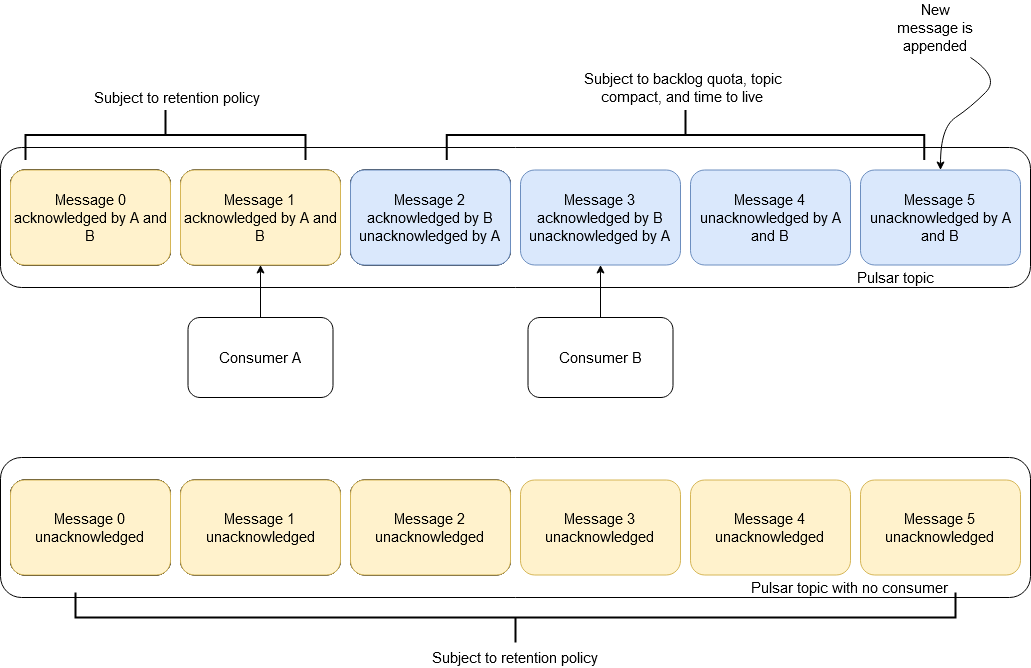
\includegraphics[width=\linewidth]{images/pulsar-retention.png}
	\caption{Message retention policy on Pulsar.}
	\label{fig:pulsarretention}
\end{figure}

By default, messages of the first type will be deleted the next time Pulsar does cleanup. Pulsar can be configured to retain these messages using retention policy \cite{pulsarretention}. User can set a time limit or a size limit for the retained messages on the topic. Whenever this limit is exceed, old messages will be deleted to keep the messages always within the limit. The size and time limits can be configured to be unlimited as well.

The second type of messages will always be retained by default. However, their size can grow too large. This can be controlled using backlog quota or time to live (\acrshort{ttl}).

The backlog quota sets a size limit on allowed unacknowledged messages of a topic. If this limit is exceeded, user can choose to reject new write request to topic or delete oldest unacknowledged messages. The main purpose of this configuration is not to save disk space. It aims at regulating the sending rate of producer in case slow consumers fall behind when consuming new messages by rejecting new sending request or reduce the number of unread messages.

On the other hand, TTL option focuses on saving the disk space. It sets a living time for unacknowledged messages. When the time expires, messages will be auto acknowledged to be subject to delete. 

Pulsar also provides the option for topic compaction \cite{pulsarconceptcompact}. However, this is completely unrelated to saving disk space and in fact will increase the disk usage. In the compaction process, Pulsar will scan through the unacknowledged messages and make a new copy containing only latest message of each key value. Messages without key values will be overlooked by the compaction process. This new compacted copy can be read by consumer when only latest values are relevant to speed up the processing.

These retention policies are only relevant to Pulsar consumer with its acknowledgement mechanism. In case of Pulsar reader, it does not acknowledge the consumption of messages to Pulsar and therefore does not determine which messages will be retained or deleted.

In summary, by default, messages on Pulsar will be deleted after being consumed by Pulsar consumer. However, it can be configured to retain messages as long as needed. Moreover, there is no option to selectively keep only latest messages to save disk space.

\large \textbf{NATS Streaming}\\
\normalsize
\textbf{Durable storage}

NATS streaming provides a pluggable persistence layer for durable storage of messages \cite{natsconfiguring}. However, by default, persistence storage is disabled and NATS streaming server only stores messages in-memory. NATS Streaming must be explicit configured to use durable storage. 

There are currently two storage options supported out-of-the-box which are file store and relational database store which is referred as SQL store in the NATS document. With file store, messages are stored in files on the disk of the server or in a network filesystem (NFS) mounted on the server. A directory is created for each channel in which messages of that channel are stored in log files. On the other hand, with SQL store, messages are persisted as records in an external relational database. All messages published to NATS Streaming are persisted in a messages table and each of them is uniquely identified by the ID number of the channel to which it belongs and an incremental sequence number. With these two provided storage options, once the producer of a message receive acknowledgement from the server, it is guaranteed that the message is durably persisted. Moreover, NATS Streaming also provides a storage interface which can be self-implemented by user to connect NATS to a different data store. 

\textbf{Event storage is fault tolerant}\\
NATS Streaming has two different clustering modes \cite{natsstreaming}. In fault tolerance mode, all server instances are mounted to the same shared data store such as \acrshort{nfs} or a shared database depending on which persistence layer is used by the servers. NATS Streaming does not support data replication for fault tolerance of data with this mode. The shared data store can become the single point of failure. Once it goes down, data is not accessible or even worse lost. If fault tolerance of data is required, it relies entirely on users. For instance, users can implement data replication on the persistence layer themselves or use a fully managed storage service such as Amazon Elastic File System. 

Fault tolerance of event store is provided out-of-the-box by NATS Streaming with the clustering mode. In this mode, each node maintains a full copy of data in a separated data store. The nodes in NATS streaming cluster use Raft Consensus algorithm to replicate data \cite{raftalg}. Only the Raft leader node can take care of receiving requests for all channels and make copies on other nodes. Users only have to start up a NATS streaming cluster with a number of nodes and data will be auto replicated among them. Producers of message will receive acknowledgement once the replication process is finished. With Raft Consensus algorithm, a cluster with \emph{2n+1} node can tolerate up to \emph{n} node failures and continue to operate while guaranteeing no message loss. If there are more failures, the NATS Streaming cluster cannot accept new messages. It is recommended by NATS to limit the cluster size to only 3 or 5 nodes.

\begin{figure}[h]
	\centering
	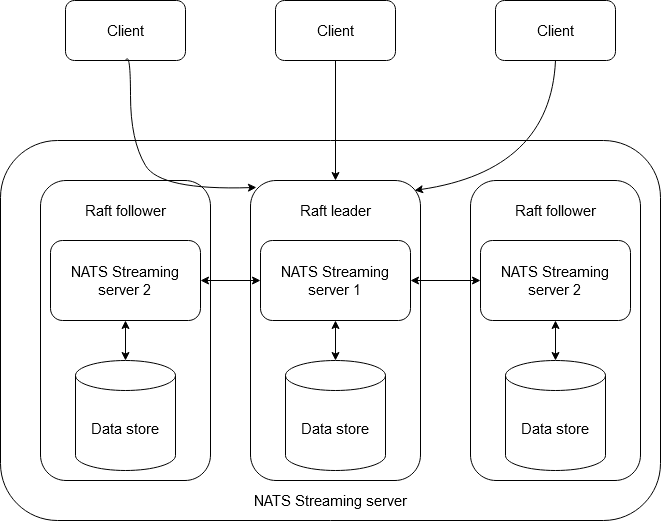
\includegraphics[width=11.5cm]{images/ft-eventstorage-nats.png}
	\caption{Fault tolerance of event storage on NATS Streaming in clustering mode.}
	\label{fig:natsftstorage}
\end{figure}

\textbf{Flexible data retention policy}\\
If persistence storage is enabled, all messages published to NATS Streaming will be retained whether they are consumed or not. User can specify the maximum number of channels, maximum size or number of messages of a channel, maximum retained time of each message \cite{natsconfiguring}.

When the limits are exceeded, oldest messages will be deleted until the retained data falls below the maximum limitation. All of these policies can be set to unlimited to retain messages forever. However, there is no option to selectively retain messages on NATS Streaming server.








\section{Messaging patterns}
\large \textbf{Apache Kafka}\\
\normalsize
Records on a Kafka topic can be read using Kafka consumer \cite{kafkaconsumer}.  Each consumer belongs to one consumer group. A topic on Kafka can be simultaneously consumed by multiple consumer groups, each of which will receive all messages from that topic. 
 
A consumer group can comprise of multiple consumers and each message on the subscribed topic will be delivered to only one of them. The important point is that the messages are not distributed randomly to consumers in the group. Instead, each partition of the topic is assigned to one consumer in the group. At any time, each partition will be assigned and read by only one consumer in the group. 

Each new record appended to a partition is assigned an offset number to be uniquely identified. This offset number is also used by Kafka consumer to indicate its current reading position on the partition. Unlike many traditional messaging systems, Kafka uses pull model to deliver messages to consumer \cite{kafkaconsumer}. That means Kafka broker does not keep track of what has been consumed by consumer with acknowledgement and therefore does not actively deliver unread messages to consumer.  It is the responsibility of consumer to provide an offset number indicating its current reading position on every request to pull new batch of messages from that point onward from Kafka. With this approach, the consumer has full control about its reading position. For durability of the consumption status, Kafka supports automatic or manual committing the offset numbers of consumers to internal Kafka topics. Consumer also can maintain its reading position in a different durable storage such as an external relational database.

\textbf{Publish-Subscribe}\\
It is very straightforward to realize the publish-subscribe pattern with the concept of consumer group of Kafka. New subscriber for a topic can be created by creating a new consumer group with only one consumer and all messages on all partitions of that topic will be delivered to this subscriber.

\textbf{Competing consumers}\\

\begin{figure}[h]
	\centering
	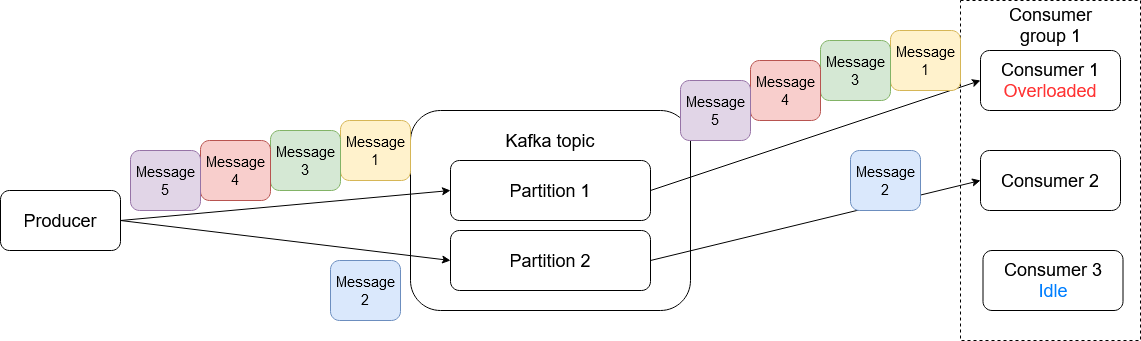
\includegraphics[width=\linewidth,height=5cm]{images/competing-consumers-kafka.png}
	\caption{Competing consumers pattern with Kafka.}
	\label{fig:kafkacompetingconsumer}
\end{figure}
The competing consumers can be realized using consumers within the same group. By adding multiple consumers to one group, they can concurrently consume messages of the subscribed topic and each message will only be read by one consumer. However, since the partition is the unit for parallel consumption in one consumer group, the number of competing consumers will be limited by the number of partitions of the topic. If there are more consumers in the group than partitions, some consumers will be unoccupied. More partitions can allow more parallel consumers. However, if there are too many partitions, this could degrade the performance of the system \cite{kafkapartitionsnum}.

Moreover, if the messages are not evenly distributed across the partitions with some retain more messages than the others, some consumers will have to handle more workload while the others are assigned with empty partitions will remain idle. Therefore, the competing consumers pattern provided by Kafka is quite rigid and cannot be scale freely.

\textbf{Publish-Subscribe + Competing consumers (Consumer group)}\\
Although it can be used as either publish-subscribe or competing consumers pattern for normal messaging scenarios, the concept of consumer group and partition itself is a combination of both these patterns provided by Kafka specifically for the event-driven use cases. By assigning each partition of a topic to a consumer in the consumer group, events of the same type published to the topic can be read and processed in parallel. 

Kafka provides a forwarding mechanism on the producer side to guarantee that events from the same entity will be delivered to the same consumer. Messages in Kafka have the key-value form. If message key is defined, it will be used to create a hash value which will then be used to determine the destination partition of the message. When an identifier is assigned to each event source and used as the key for published events, these events will end up in the same partition on the destination topic. As a result, the consumption of events can be scaled by tuning the number of partitions and consumers in the group while ensuring that each consumer will receive the entire history of events from a specific entity.  

\begin{figure}[h]
	\centering
	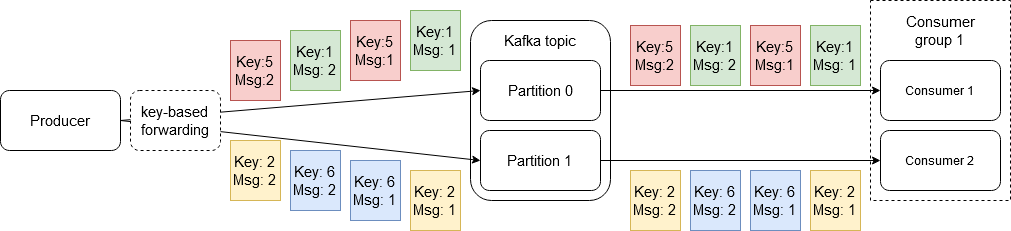
\includegraphics[width=\linewidth,height=4cm]{images/consumer-group-kafka.png}
	\caption{Consumer group pattern with Kafka.}
	\label{fig:kafkaconsumergroup}
\end{figure}


\textbf{Consumer group failover mechanism}\\
Consumers in the group periodically send heartbeats to Kafka to indicate their liveness. Moreover, they must also regularly send new requests for messages from Kafka. If a consumer fails to meet either condition, it is considered to be failed and will be removed by Kafka from the group \cite{kafkaconsumerimplement}. 

In case a consumer fails, its partitions will be reassigned to other consumers in the group automatically. The failover consumer will continue to process messages from the latest reading position of the failed consumer. If this reading position is checkpointed in Kafka, the task of retrieving the consumption status of failed consumer and sending it to the taking-over consumer will be managed transparently by Kafka. On the other hand, if the failed consumer persists its position in an external datastore, Kafka provides the callback \emph{ConsumerRebalanceListener} for consumer to determine when partition rebalancing occurs and retrieve the last reading position on newly assigned partition.

\textbf{Event playback}\\
A Kafka consumer must specify its reading position using offset number in every request to pull new messages from Kafka. Therefore, it is very straightforward to re-consume older records in Kafka by simply using an older offset number for the new consuming request. 

\begin{figure}[h]
	\centering
	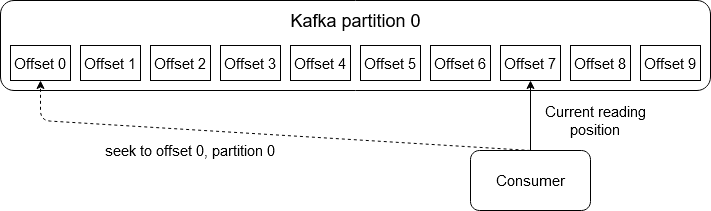
\includegraphics[width=10cm,height=4cm]{images/event-playback-kafka.png}
	\caption{Event playback with Kafka.}
	\label{fig:kafkaeventplayback}
\end{figure}

By default, if a consumer is started with an existing consumer group, its reading position on the assigned partition starts from the latest committed offset number on either Kafka or external datastore, and the position will advance after every request for new messages. However, a Kafka consumer can also reset its reading to an arbitrary position \cite{kafkaconsumerimplement}. This reset operation is done on partition basis. A consumer can only reset the offset of partitions that it is currently assigned to. Next time the consumer pulls more records from this partition, it will start from the reset offset position.

\large \textbf{Apache Pulsar}\\
\normalsize
There are two ways to consume message from Pulsar, namely, using Pulsar consumer and Pulsar reader.

The consumption of messages with Pulsar consumer is quite similar to traditional messaging system. Pulsar uses a combination of push and pull models to deliver messages to consumer \cite{pulsarbinaryprotocol}. Acknowledgment must be sent back to Pulsar broker upon successful processing of a message. The broker will keep track of the consumption status of consumers and will send unacknowledged messages to a queue on the consumer side when it receives permission from the consumer. Messages on this queue is dequeued and consumed gradually by the application. Once the queue is halved, Pulsar consumer sends a new request for new messages to be pushed to the queue again. Moreover, Pulsar broker also uses the acknowledgements to mark messages as being able to be deleted.

Consumers subscribe to a topic by creating a subscription \cite{pulsarconsumersubscription}. Multiple consumers can be grouped together with the same subscription to consume messages on the topic together. There are four different subscription modes, namely, Exclusive, Failover, Shared and Key\_Shared each of which is relevant to a different messaging pattern supported by Pulsar. However, with the current release of Pulsar, the Key\_Shared subscription mode is still unstable \cite{pulsarkaysharedunstable}. Therefore, this mode will not be considered further in the thesis.

On the other hand, the Pulsar reader is internally a Pulsar consumer with special configurations \cite{pulsarreader}. The Pulsar broker does not monitor the consumption status of reader and does not require acknowledgement of messages. Therefore, Pulsar broker does not control which messages to be delivered to reader. On starting up, the reader must define a specific starting position by giving the ID of the first message to be read and only messages from that point onward will be delivered to the reader. This reader is designed to give users more control over which messages to be read from Pulsar and is quite similar to Kafka consumer. If the reader needs durable consumption status, it has to maintain its own current reading position in a durable storage and manually retrieve that on every startup. Pulsar does not support auto-checkpointing reader position natively on Pulsar as in Kafka. 

However, there is no possibility like subscription to group multiple readers together. Each reader connects directly to a topic and starts consuming all messages individually. Therefore, it is not possible to realize messaging patterns of shared consumption such as competing consumers and consumer group with Pulsar reader. Moreover, at the moment with Pulsar 2.7.0, a Pulsar reader can only read from non-partitioned topics.

\textbf{Publish-Subscribe}\\
Pulsar provides the Publish-Subscribe pattern with the Exclusive subscription mode of consumer. In this mode, at any time, only one consumer is allowed in the subscription, other consumers which join the subscription later will be rejected. All messages on the subscribed topic will be delivered to the single consumer in the subscription. Different subscribers can create a new exclusive subscription to the topic with different subscription names.

The publish-subscribe pattern can also be realized with the Pulsar reader. Multiple readers on a non-partitioned topic can simply be started and every message on the topic will be delivered to all of them. 

\textbf{Competing consumers}\\
This pattern is realized on Pulsar with the Shared subscription mode. Multiple consumers can be grouped together using this mode. Messages will be distributed to the consumers in a round-robin fashion and each message will be delivered to only one consumer in the group.

\textbf{Publish-Subscribe + Competing consumers (Consumer group)}\\
Like Kafka, messages on Pulsar have the key-value form. If a message is created without a key, it will be delivered to a random partition of the topic. But if a key value is assigned, its hashed value will be used to determine the target partition for the message on the topic. On Pulsar, to enable the combination of Publish-Subscribe and Competing consumers, on the producer side, key values must be assigned to all generated events. They will be used as identifiers for events from the same source and help deliver them to only one consumer.

On consumer side, Failover subscription mode can be used to realize this pattern. In this mode, multiple consumers can be grouped together into the same subscription. Each partition of the subscribed topic will be assigned to only one consumer in the group. Only if a consumer fails, its partitions will be taken over by another consumer in the subscription. By adding key to each event on the producer side, it is ensured that events of the same entity will be on the same partition and therefore a consumer in the subscription will receive all of them. This is similar to the consumer group in Kafka and it requires the topic to be partitioned to enable this parallel consumption. The level of parallelism is also limited by the number of partitions of the topic. 

\begin{figure}[h]
	\centering
	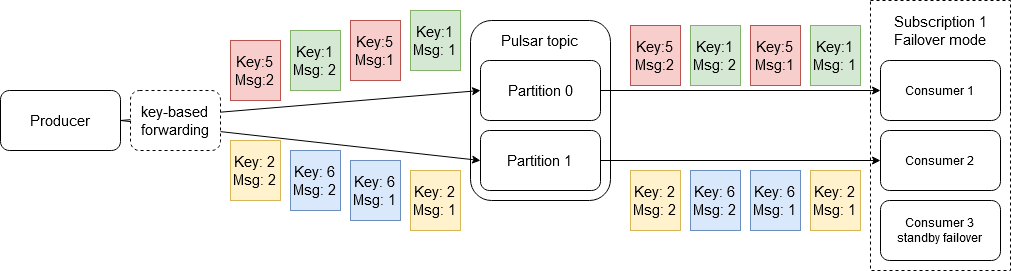
\includegraphics[width=\linewidth,height=4cm]{images/consumer-group-pulsar.png}
	\caption{Consumer group pattern with Pulsar.}
	\label{fig:pulsarconsumergroup}
\end{figure}

\textbf{Consumer group failover mechanism}\\
In Failover mode, each partition of the topic is assigned to one consumer in the subscription. Pulsar broker automatically monitors the connection to every consumer. 

If a consumer disconnects, its partitions will be assigned to other consumers automatically by Pulsar. Moreover, because Pulsar broker keeps track of the consumption statuses of all consumers with acknowledgment, it will know which messages have not been read by the failed consumer and continue to deliver them to the failover consumer.

\textbf{Event playback}\\
For Apache Pulsar, event playback is possible with both Consumer and Reader API.

Pulsar consumer must acknowledge the consumption of each message. It is the responsibility of the broker to decide which messages will be delivered based on the acknowledgments received from the consumer. By default, if a consumer is started with an existing subscription, the reading will automatically be started from the earliest unacknowledged message onward. Nevertheless, it is also possible to reset the consuming position of the subscription with Consumer API \cite{pulsarconsumerapi}. User can reset reading position to a message with a specific message ID. The message ID must be known beforehand. It is also possible to reset the reading position of the subscription to message published at the time equal or greater than a specified timestamp. 

With Pulsar reader, a starting position of messages to be read from the topic must be specified every time it is started. As a result, the reader has the flexibility to jump to arbitrary positions and replay events on the topic whenever needed \cite{pulsarreaderapi}. The starting position can be defined by providing a message ID. User can also specify a rollback duration to rewind the reading position to a specific time point. The times semantics of both consumer and reader is when the messages were published and were automatically assigned by the Pulsar producer.
\begin{figure}[h]
	\centering
	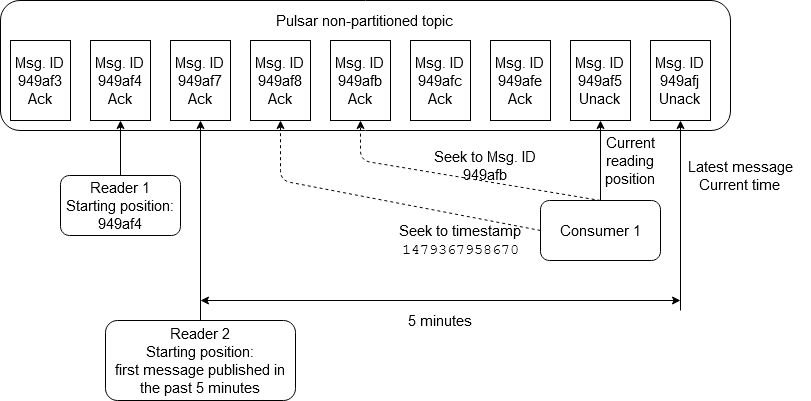
\includegraphics[width=\linewidth,height=5cm]{images/event-playback-pulsar.png}
	\caption{Event playback with Pulsar.}
	\label{fig:pulsareventplayback}
\end{figure}

\large \textbf{NATS Streaming}\\
\normalsize
With NATS Streaming client API, a consumer must create a subscription to a channel to be able to start consuming messages \cite{natssubscription}. NATS Streaming provide two subscription modes. The first is normal mode which means there is only one consumer per subscription, and it will receive all messages on the channel. The second mode is queue mode where a subscription has multiple competing consumers which will read the same topic and each message will be read by only one consumer. 

NATS streaming uses push model to deliver messages to subscriber. That means the server controls which messages to be sent to consumer. The server keeps up with the current consumption status of each consumer by receiving acknowledgments. NATS server actively pushes next unacknowledged messages to the consumer and expects that the receiving application is available to process these messages right away. Consumer must acknowledge with server about the successful consumption of every message within a predefined time window. Otherwise, unacknowledged messages will be redelivered to subscriber after timeout. 
 
By default, NATS server only retains the consumption status of a consumer during the connection session. When being disconnect, the current reading position of the consumer will not be remembered by the server. In this case, if the consumer wants to resume its consumption from the previous session, it must maintain its own reading position in an external storage and provides it as the starting position to read when reconnecting to the server. 

To have a durable consumption status on the server which will be automatically resumed when the consumer reconnects, the subscription must be strictly configured to be durable. When a subscriber starts consuming messages using an existing durable subscription, it will resume its consumption of the unacknowledged messages from the previous connection session.

\textbf{Publish-Subscribe}\\
In NATS Streaming, a new subscriber to a channel can be set up by simply starting a consumer in normal mode with a new client ID and all messages on that channel will be delivered to this new consumer. 

\textbf{Competing consumers}\\
Competing consumers for a topic can be grouped together into a subscription with queue mode. NATS Streaming will deliver messages to consumers in the group randomly and each message will be sent to only one consumer. The number of consumers in a queue group can be scaled freely.

\textbf{Publish-Subscribe + Competing consumers (Consumer group)}\\
NATS Streaming offers no combination of Publish-Subscribe and Competing consumers patterns. The subscriber in Publish-Subscribe pattern is not scalable. On the other hand, with the competing consumers pattern, it is not guaranteed that all events from one source will be delivered to the same consumer because of the random distribution of message in the group. If parallel consumption of events is needed, it must be self-implemented by user on the channel level. In this case, all the task of partitioning events of the same type into multiple channels, forwarding events from the same source to the same channel and assigning each channel to one subscriber will have to be done manually.

\textbf{Consumer group failover mechanism}\\
Since the consumer group pattern is not supported by NATS Streaming, there is also no failover mechanism.

\textbf{Event playback}\\
Event playback with NATS Streaming is very straightforward. When creating a subscriber to a NATS channel, user has the ability to choose different starting positions for the subscription \cite{natseventplayback}. Consumer can start consuming messages from a specific sequence number on the channel, from a specific starting time or from a rewind duration. The time semantics here is when a message is stored on the NATS server and is managed by the server.
\begin{figure}[h]
	\centering
	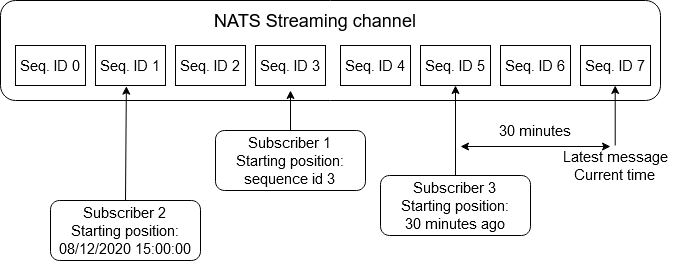
\includegraphics[width=\linewidth,height=5cm]{images/event-playback-nats.png}
	\caption{Event playback with NATS Streaming.}
	\label{fig:natseventplayback}
\end{figure}

By default, the subscription on NATS Streaming is not durable. Thus, when a subscriber disconnects to the server, its current reading position will be lost. As a result, user can choose a different starting position every time the subscriber is restarted and can freely jump to different messages on the channel. In case of durable subscription, the current reading position of the subscriber is kept track by the server. Therefore, to replay events, subscriber must first unsubscribe the durable subscription before it can specify a new reading position using the same subscription name.








\section{Messaging semantics} \label{section:semantics}
In systems with asynchronous messaging, messaging semantics such as ordering guarantee, delivery guarantee cannot be provided by the message broker alone. The producers and consumers of messages must collaborate with the messages broker to achieve different levels of semantics. Therefore, in this section, before going into the evaluation, the general prerequisite for collaboration of the clients, which is true for all ESP platforms, is briefly recapped.
\subsection{General prerequisite}
\textbf{Strong ordering guarantee}\\
To achieve ordering guarantee of messages, the throughput must be compromised. On the message publishing side, at any time, messages from the same source must be published from only one producer instance. Otherwise, since concurrent producers publish events independently and are subject to different network conditions, the order of events cannot be preserved when they arrive at the ESP platform. Similarly for consumers, to guarantee that messages from the same source are processed in the correct order, concurrent consumption with multiple application instances is not permitted.

To have both concurrency and ordering guarantee, the concurrent instances must coordinate with each other to enforce the right order when publishing or consuming messages. Nevertheless, this method can introduce more overhead to the system.

Moreover, when a producer asynchronously send a message and proceed to the next one before receiving acknowledgement from the broker, if a message fails to reach the broker and is resent later, it is possible that another message may arrive in between causing their orders to be interchanged (figure \ref{fig:outorderretry}).
\begin{figure}[h]
	\centering
	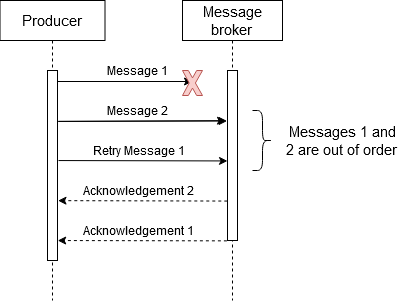
\includegraphics[width=10cm]{images/order.png}
	\caption{Asynchronous publishing and retrying causes out-of-order messages.}
	\label{fig:outorderretry}
\end{figure}

Therefore, in case the broker does not support detect out-of-order of asynchronously published messages, producer should only synchronously publish message one by one for ordering guarantee.


\textbf{At-most-once and At-least-once delivery semantics}\\
When a message is published, it can be lost along the way from producer to broker. Therefore, it is the responsibility of the producer to keep tracks of the sending status and resend messages if necessary. On the receiving side, after receiving and processing a message received from the broker, a consumer usually must perform two operations, namely, durably persisting the result of the processing and updating the current reading position on the source message stream to indicate that it has finished with the current message and will not receive it again. Since failures can non-deterministically occur between two operations, different order of these operations can result in different delivery guarantees. 

With at-most-once semantics, a producer can simply send messages in a fire-and-forget fashion without waiting for acknowledgements of successfully receiving from the message broker. Therefore, one of the key benefits of at-most-once guarantee is higher throughput since the producer is not impeded by the overhead introduced by acknowledging. When failures occur, messages may not reach the platform and are lost. When consuming a message, consumer must update its current reading position \underline{before} committing the calculated result from the message. In this way, if the consumer goes down before the result is persisted, it will continue with the next message upon restarting while the previous message will not be received again, and the corresponding result is simply lost.

For at-least-once semantics, messages producer must wait for acknowledgement from server for every message and is responsible for resending to avoid message loss. As a result, within one connection session, a message can appear on the message pipeline multiple times in case it is already received by the broker but the acknowledgement to the producer is lost. On the consumption side, for each received message, the consumer must mark it as being consumed and update the reading position only \underline{after} it has handled the message and durably persisted the result. In this way, if the consumer crashes after the result is stored but before the current reading position is updated, it will receive and process the message again after restarting and a new result will be generated along with the previously persisted result. In this case, duplication will be introduced between two connection sessions.
\begin{figure}[h]
	\centering
	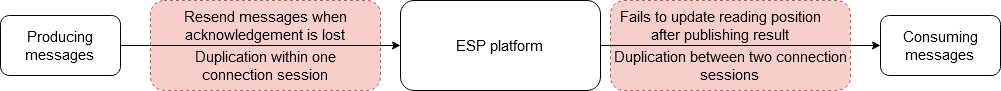
\includegraphics[width=\linewidth]{images/at-least-once-duplication.png}
	\caption{Duplication of messages with at-least-once delivery semantics.}
	\label{fig:messageduplication}
\end{figure}

\textbf{Exactly-once semantics}\\
Although it is physically not possible to ensure that each message is delivered and processed exactly once in a distributed system given the non-reliable nature of network \cite{exactlyoncenotpossible}, exactly-once processing semantics can still be realized on top of at-least-once guarantee. 

With at-least-once semantics, duplication can be introduced within one connection session or between two consecutive connection sessions. One possible solution is having the processing logic of the application to be idempotent so that multiple retries do not affect the end result. However, the feasibility of this approach depends on specific use cases.

Another approach is implementing deduplication mechanism on either the client or the message broker. The evaluation will focus on inspecting the support of this feature on the ESP platforms. 

\subsection{Evaluation}
\large \textbf{Apache Kafka}\\
\normalsize
\textbf{Strong ordering guarantee}\\
A Kafka topic comprises of one or more partitions. Kafka can guarantee that when two records are written to the same partition, they will be stored and delivered to consumers in the same order as their arriving order \cite{kafkaconfluentintro}.

On the consumer side, in a Kafka consumer group, each partition of the topic is assigned to only one consumer. There are no other competing consumers for each partition. As a result, the delivery model of Kafka guarantee that messages on a partition are delivered and processed in the right order.

On the producer side, all events from the same source must be sent to the same partition where order is guaranteed by Kafka. By default, records with the same key value will be published to the same partition. Therefore, producers must assign appropriate key value for each published message.

Asynchronous publishing of messages while ensuring order is also possible with Kafka. From Kafka 0.11, the idempotent producer is introduced \cite{kafkatransaction}. When this feature is enabled on a producer, for each targeted partition, each writing request will be assigned an incremental sequence number which will be used for deduplication on the broker in case of retrying. Thanks to this sequence number, Kafka can also tolerate up to 5 asynchronous publishing requests from one producer.

\textbf{At-most-once and At-least-once delivery semantics}\\
With Kafka producer, users have the flexibility to control the level of durability of published messages. Producer can be configured to wait for acknowledgements from only the leader partition, from all in-sync replicas or not wait for any confirmation from Kafka broker at all \cite{kafkaconfigurationproducer}. For the at-most-once guarantee, producer can be configured to send a record and immediately proceed to the next one without waiting for acknowledgement from the server. With the at-least-once guarantee, durability of published message must be ensured. Therefore, as elaborated in section \ref{section:eventstorage}, the producer must be configured to wait for the acknowledgements from all in-sync replicas to ensure that the published message is safely received and replicated by the Kafka server. Internally, if Kafka producer is configured to wait for acknowledgement from brokers, it will retry in case of failure until timeout. Therefore, there is no need to implement the retry logic in the application. 

On the Kafka consumer, by default, the offset number indicating the current reading position will be periodically persisted to Kafka. To have a better control over when to update the reading position, this should be disabled. The offset number should be manually committed before or after persisting the calculated result depending on the chosen delivery semantics.   

To sum up, Kafka supports both at-most-once and at-least-once delivery semantics with its clients.

\textbf{Exactly-once semantics}\\
From release 0.11 \cite{kafkatransaction}, Kafka provides mechanisms to protect against both types of duplication introduced by at-least-once semantics (figure \ref{fig:messageduplication}) and realize exactly-once semantics. 

To avoid duplicated messages by producer resending, the idempotent producer is introduced. Whenever a new producer instance is created and connected to Kafka, it is assigned a unique ID by the broker. When publishing messages to a partition, producer will add an incremental sequence number to every message along with its ID. By using these two values, the broker can uniquely identify a specific message sent by a producer on each partition and can discard any duplicated messages resulted from resending. 

To prevent duplication across two different connection sessions, Kafka provides the transaction feature. When a Kafka producer writes records to multiple partitions in a transaction, either all produced records are safely persisted or none of them is available to be read by other Kafka consumers. When Kafka consumer persists its current reading position to Kafka, internally this value is written to a special Kafka topic. Therefore, the act of updating reading position can be put in a transaction similarly to producing a normal record.

\begin{figure}[h]
	\centering
	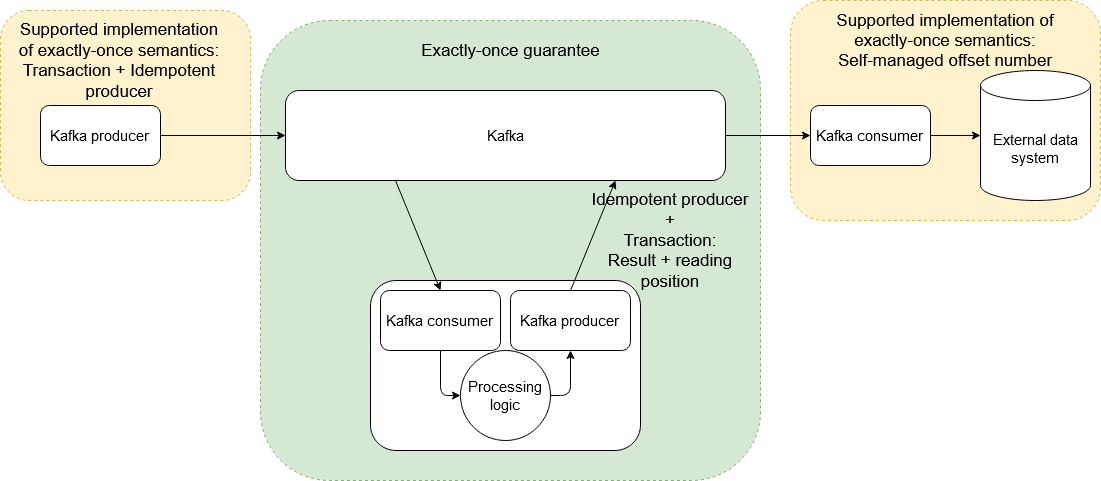
\includegraphics[width=\linewidth]{images/exactly-once-kafka.png}
	\caption{Support of exactly-once semantics on Kafka.}
	\label{fig:exactlyoncekafka}
\end{figure}


For application which obtains data from Kafka topics with Kafka consumer and then produces new records back to Kafka, it can use Kafka producer to persist the result to output topics and commit the current reading position on input topics in a single transaction. In this way, even if the application crashes while producing records back to Kafka, when it restarts, it can start consuming records again from a clean state with the latest successfully committed result and reading position. Any result generated in the middle of a failed transaction will be discarded. 

In case of edge application which obtains data from an external system and produces records to Kafka, the application can produce records along with their related reading positions on the external system in a transaction. Upon restarting, application can retrieve the last committed position on Kafka and resume the processing on the external system accordingly. 

However, for edge consuming application which will write result to an external system, the transaction cannot span across its Kafka boundary. In this case, one possible approach is persisting atomically the reading position of the consumer along with the calculated result in the targeted external data system given that it supports transactions. Upon restarted, the consumer can retrieve the committed offset number and resume consumption accordingly. The delivery model of Kafka makes it easier to implement this since the reading position is only an offset number and can be controlled and persisted anywhere by the consumer.


\large \textbf{Apache Pulsar}\\
\normalsize
\textbf{Strong ordering guarantee}\\
A topic on Pulsar can either be non-partitioned or partitioned. Internally, a partition is also a normal non-partitioned topic. Pulsar guarantees that messages published to the same partition/non-partitioned topic will always be delivered to consumption side in the order in which they arrived at Pulsar \cite{pulsarconceptmessaging}.

If Pulsar consumer is used to consume messages, the Explicit and Failover subscription mode can be used to ensure the order of arriving messages. In the Explicit mode, there are no competing consumers for a topic regardless of being partitioned or not. With the Failover mode, similarly to Kafka consumer group, each partition will be assigned to only one consumer in the subscription while other consumers only take over when failures occur. Thus, each consumer in these two modes can receive all messages on a partition from Pulsar in the right order. If Pulsar reader is used, order of consumed messages is guaranteed since each reader can only be connected to a non-partitioned topic and grouping multiple readers for parallel reading of a topic is not possible. 

On producer side, if the topic is partitioned, appropriate key values must be assigned to every message to ensure that events from the same source will be produced to the same partition where order of delivery is guaranteed by Pulsar.

Regarding asynchronous publishing of messages, Pulsar also claims that a producer can have multiple asynchronous requests on the same connection to Pulsar while the order of messages received on the broker is still guaranteed \cite{pulsarinflight}.

\textbf{At-most-once and At-least-once delivery semantics}\\
When using Pulsar producer, it is not possible to publish messages in a fire-and-forget way. Internally, the producer always waits for confirmation from the broker and retries sending the messages if no acknowledgement is received until a specified timeout. As a result, a message can be duplicated on the stream. The Pulsar broker supports deduplication of resent messages. However, this will introduce overheads on both the producer for resending and the brokers for deduplication which does not comply with the key benefit of low overhead of at-most-once semantics. Therefore, in general, Pulsar producer does not support at-most-once. On the other hand, the Pulsar producer is very suitable for the at-least-once guarantee. Since the producer always waits for acknowledgement and retries sending message internally, no self-implementation of retry logic is needed.  

On the consuming side, the application must update the reading position (by either acknowledging if Pulsar consumer is used or persisting message ID of the consumed message if Pulsar reader is used) and durably persist the calculated in the appropriate order for the delivery semantics.

Considering both publishing and consuming sides, Pulsar clients only support at-least-once delivery semantics.

\textbf{Exactly-once semantics}\\
From release 1.20.0, Pulsar provides idempotent producer to discard any duplicated message introduced by producer retrying \cite{pulsaridemproducer}. With this feature, each producer must be assigned a globally unique name. Each message published to a Pulsar topic will be automatically assigned an incremental sequence ID by the producer. Pulsar broker will use the producer name and the sequence ID to uniquely identify each message published by a producer on a topic and discard any duplicated message resulted from retrying. 

For deduplication of duplicated messages created by consumer between two connection sessions, from release 2.7.0, Pulsar provides the transaction feature for Pulsar producer and consumer \cite{pulsartransaction}. With this new feature, users can publish messages to multiple Pulsar topics as well as acknowledge consumed message on numerous Pulsar source topics in one atomic operation. If the application fails during the transaction, all half-committed values will be discarded.  

For application which reads messages from Pulsar and produces results back to Pulsar, exactly-once semantics can be achieved. The transaction feature can be used to ensure that the application will always recover from a crash with a clean state on both source and output Pulsar topics.   

For application which processes data on external system and produces messages to Pulsar, it can use Pulsar producer to send messages and the corresponding reading positions on the external system to Pulsar in one transaction.  In this way, the application can resume the consumption on the external system after failure with the committed position on Pulsar to ensure the exactly-once semantics. 

In case of application which reads messages from Pulsar and writes result to an external system, the Pulsar transaction cannot span on both systems. In this case, exactly-once must be self-implemented. For instance, the Pulsar transaction can be integrated into the two-phase commit protocol \cite{twophasecommit} to acknowledge consumed messages on Pulsar and produce new messages to external system. This approach is used in the implementation of this connector to connect Apache Pulsar and Apache Flink \cite{pulsarflinkconnector}. However, this method depends on the availability of support for two-phase commit on destination system. Users can also use Pulsar reader to have more flexible control on the reading position on Pulsar. In this case, the message ID of the currently consume message on Pulsar can be persist together with the corresponding result to the external system to achieve atomicity similarly to Kafka.

The transaction feature is still in technical review phase. Therefore, this feature should not be used for production and exactly-once semantics is considered to be only partly supported on Apache Pulsar at the moment.


\begin{figure}[h]
	\centering
	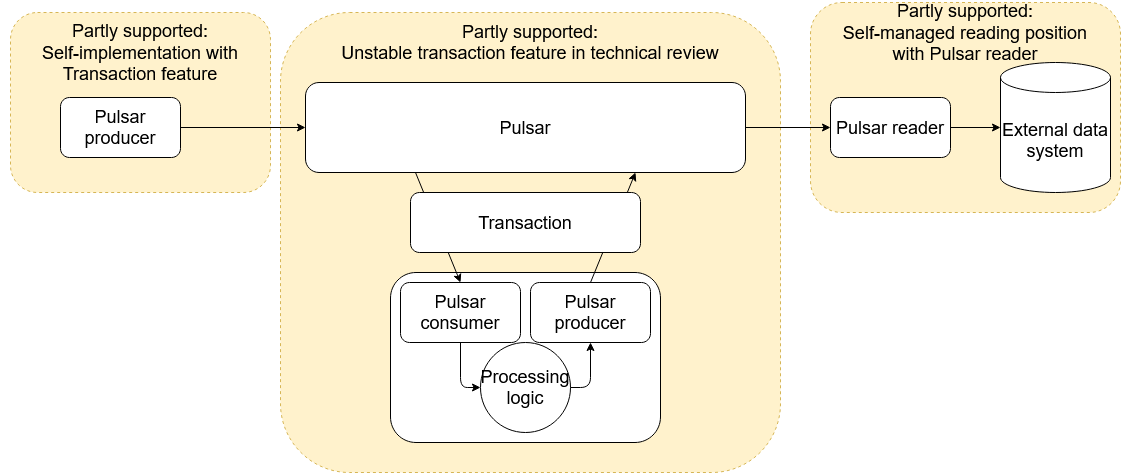
\includegraphics[width=\linewidth]{images/exactly-once-pulsar.png}
	\caption{Support of exactly-once semantics on Pulsar.}
	\label{fig:exactlyoncepulsar}
\end{figure}




\large \textbf{NATS Streaming}\\
\normalsize
\textbf{Strong ordering guarantee}\\
Messages on NAT Streaming are organized into different channels. There is no lower level of partitioning of messages. NATS streaming can guarantee that when a subscriber consumes from a channel, messages are delivered in the same order as when they are published and persisted to the channel. This is not explicitly written in the document, but it is explained by NATS development team in discussions on GitHub \cite{natsorder}.

On the subscriber, to guarantee the order of messages, only normal subscription mode can be used. In this mode, each subscription has only one consumer without any other competing consumer \cite{natsconceptchannels}. Therefore, this single consumer can receive all messages on the channel in right order and process them sequentially.

Moreover, with its delivery model, NATS streaming actively pushes messages to subscriber and expects that these messages will be processed right away and acknowledged shortly after. Therefore, in case the consumption of a message takes longer time than the timeout for acknowledgement, the message can be resent out-of-order along with new messages. If the processing speed of client does not match the delivery of server, the sequence of delivered messages will not retain the right order anymore (figure \ref{fig:ordernats}).


Therefore, the sending rate of the server must be limited to only one unacknowledged message at a time necessary to avoid out-of-order redelivery \cite{natsdevelopingacks}. As a result, it is not possible to receive messages in batch with NATS Streaming. 

\begin{figure}[h]
	\centering
	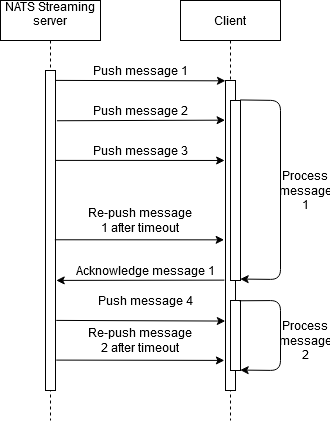
\includegraphics[width=9cm]{images/order-nats.png}
	\caption{NATS Streaming server redelivers messages out-of-order: message 1 and 2 are processed longer than the acknowledgement timeout and therefore are resent by server. Client sees the sequence of messages 1, 2, 3, 1, 4, 2.}
	\label{fig:ordernats}
\end{figure}

On the producer side, messages must be published to the same channel where order is retained. Moreover, producer must synchronously send the messages one after another since the NATS server does not support protection against out-of-order caused by resending messages.  

\textbf{At-most-once and At-least-once delivery semantics}\\
Internally NATS producer always wait for acknowledgement from server after publishing a message. However, unlike Kafka and Pulsar, this producer does not retry internally to resend a message if it does not receive acknowledgement from the server. Thus, to have at-most-once guarantee on the publishing side, the publishing status returned by the producer can be simply ignored to realize fire-and-forget publishing. On the other hand, for at-least-once semantics, returned error from the producer should be handled with self-implemented retry logic to guarantee that the deliveries of all messages are successful.

NATS subscriber must acknowledge every consumed messages so that the server can continue to push next unacknowledged messages. However, the acknowledgement by NATS client to server is fire-and-forget \cite{natsorder}. The acknowledgment can be lost without the subscriber knowing about it which will cause the the message to be resent. If a consumer can perform deduplication to process each message exactly once, end-to-end at-most-once guarantee can still be realized. Nevertheless, as will be seen in the next evaluation section, end-to-end exactly-once guarantee cannot be achieved on NATS Streaming. As a result, at-most-once delivery guarantee is also not realizable by NATS Streaming.

On the other hand, at-least-once consumption of messages is possible with NATS clients. Consumer must update its reading position (by acknowledging the message with the server for durable subscription or checkpointing the reading position to external system for non-durable subscription) after it has durably published the calculated result. In case of non-durable subscription, the consumer still needs to send acknowledgement to the server. Nevertheless, when to acknowledge is irrelevant since the consumer only relies on the external checkpoint to resume the consumption. 

\textbf{Exactly-once semantics}\\
Currently, NATS Streaming server does not support detect and discard duplication within one connection session when a client resends a message multiple time. If deduplication is needed, it must be self-implemented on the application layer. 

For duplication introduced between connection sessions when client crashes before updating its current reading position, NATS Streaming also provides no deduplication mechanism. For an application which reads messages from NATS and publishes the results to another NATS channel, it is not possible to atomically publish new message and update reading position on source channel. Therefore, it is always possible that a message whose result is already published will be re-consumed and duplicated result will be generated. The same applies to application which publishes messages obtained from an external system to NATS Streaming.

For application which consumes messages from NATS and writes results to an external storage, it can use non-durable subscription and rely on the transactional feature of the sink system to store the sequence ID of consumed message and output value to achieve exactly-once. However, NATS Streaming server can always redeliver a message when it does not receive acknowledgement from client after timeout. There are also duplicated messages introduced to the channel from the upstream applications. Application must handle the deduplication of these messages as well.

As a result, in general, exactly-once semantics is not supported by NATS Streaming.


\begin{figure}[h]
	\centering
	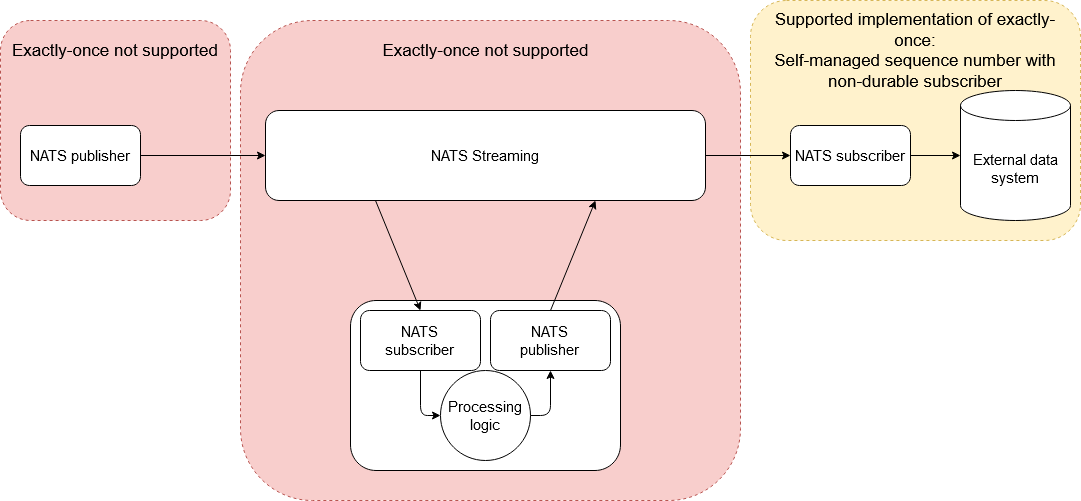
\includegraphics[width=\linewidth]{images/exactly-once-nats.png}
	\caption{Support of exactly-once semantics on NATS Streaming.}
	\label{fig:exactlyoncenats}
\end{figure}







\section{Stream processing}
\large \textbf{Apache Kafka}\\
\normalsize
\textbf{Native stream processing}\\
From release v0.10, Kafka provides the Kafka Streams to support native stream processing \cite{kafkastreams}. This is a Java library built on top of Kafka producer and consumer. Users can use this library to implement and deploy stream processor which reads input records from Kafka and produces calculated results back to Kafka as a normal Java application. 

One of the main advantages of Kafka Streams is that users does not need to set up a separated cluster for stream processing. Normal Java application instance can be simply started anywhere to do the stream processing with Kafka. Moreover, since Kafka Streams is developed from normal Kafka client, it inherits the parallelism and failover concept of the Kafka consumer group. Multiple instances of a stream processor can be started for scalability. Each instance is assigned a set of partitions from the input topics. This also guarantees that records on the same partitions are processed by only one instance in the same order as when they are sent to Kafka. When the number of instances is changed due to failure or scaling up with more instances, the partition will be automatically rebalanced similar to the Kafka consumer group. Moreover, Kafka Streams also benefits from the features of idempotent producer and transaction of Kafka client. Therefore, exactly-once processing guarantee can be achieved with this library.

Kafka Streams library provides the Streams Domain Specific Language (DSL) which supports a rich set of functionalities. The DSL provides logical abstraction of Kafka topics as \emph{KStreams} and \emph{KTables}. A \emph{KStream} consists of all records in a Kafka topic while a \emph{KTable} only presents the latest values of each record key in the topic which is similar to a normal database table. The table representation can be very useful when doing lookup of the current state of an entity. 

The DSL supports a rich set of both stateless and stateful operations on top of its abstractions. There are many stateless operations such as filtering, mapping each record to a set of corresponding outputs. For stateful processing, the DSL support aggregating multiple records to extract result, joining \emph{KStreams} and \emph{KTables}, grouping records into window for processing. Users also have the flexibility to choose the semantics for the time boundaries of the windows such as event time (i.e. the time a record is actually generated at the source) or processing time (i.e. when the records are received by the stream processor). Users also have the possibility to choose different types of windows, control how the windows are advanced over time (Figure \ref{fig:windowtypes}).

\begin{figure}[h]
	\centering
	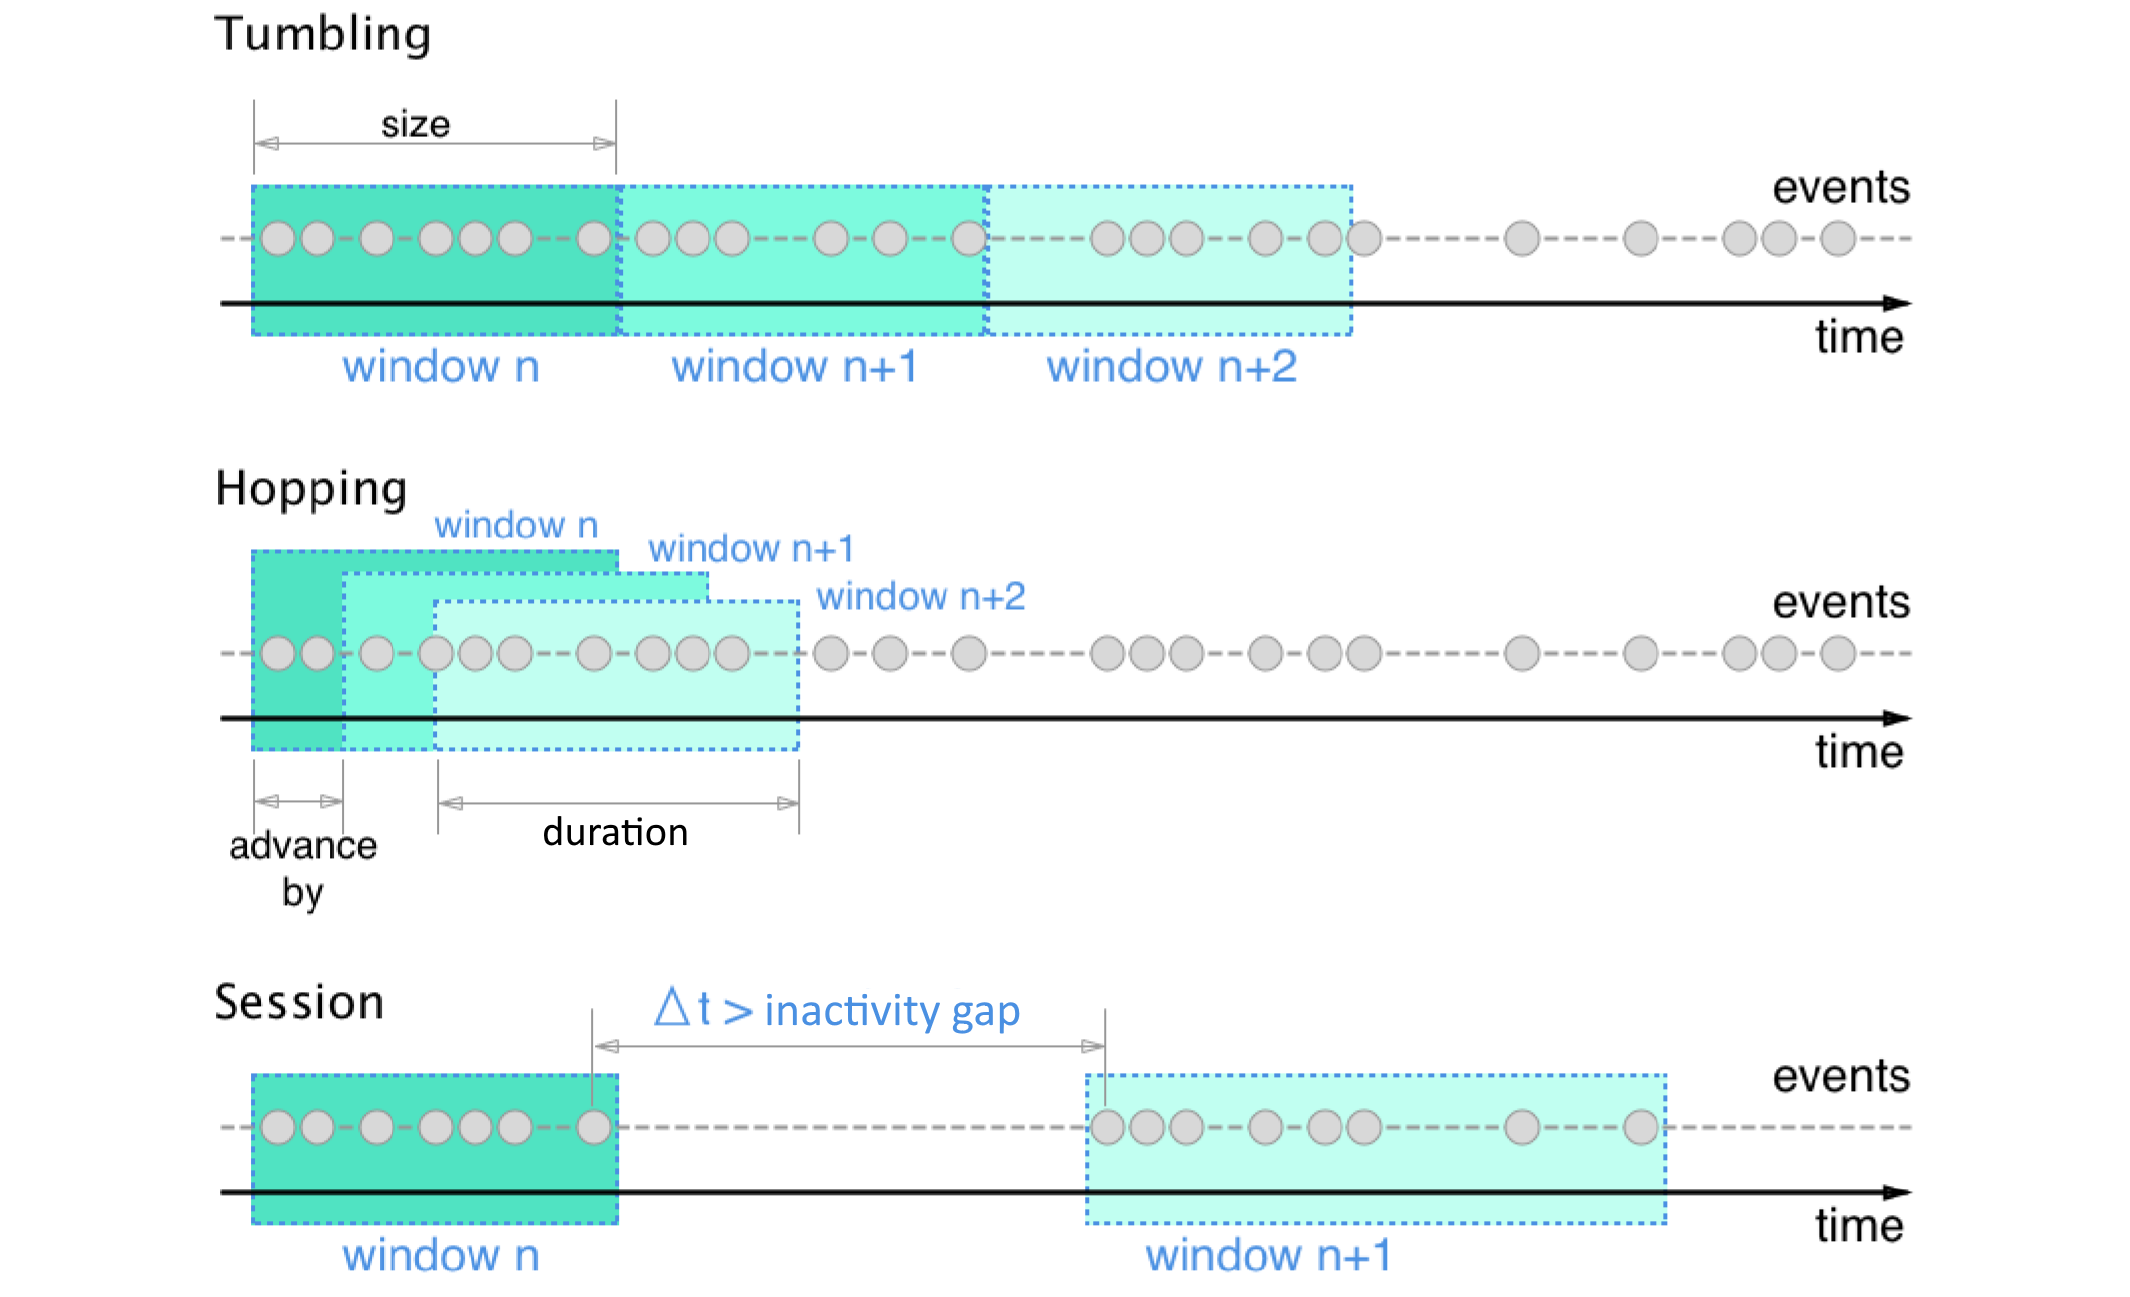
\includegraphics[width=\linewidth]{images/window-types.png}
	\caption{Supported window types for stream processing with Kafka Streams (taken from \cite{windowtypes}).}
	\label{fig:windowtypes}
\end{figure}

Each Kafka Streams application instance retains the current state of the stateful operations in a local state store. This has a number of advantages such as faster state query than remote storage, better isolation between the instances \cite{localstatestore}. Moreover, Kafka Streams also supports checkpointing the local state store to a Kafka topic for fault-tolerance which is managed completely transparent to users.

Apart from DSL, Kafka Streams also provides a lower-level Processor API. With this API, users have more flexibility to implement more sophisticated stateless and stateful operations which are not provided by the DSL. 

To sum up, Kafka Streams is a powerful tool to do stream processing on top of Kafka topics. Stream processors which are implemented using Kafka Streams not only benefit from various useful functions of the library, they can also integrate seamlessly with Kafka for scalability and fault-tolerance.





\large \textbf{Apache Pulsar}\\
\normalsize
\textbf{Native stream processing}\\
Apache Pulsar provides the Pulsar Functions for native stream processing \cite{pulsarfunction}. The concept of Pulsar Functions is similar to serverless function as a service (FaaS). Users can start a number of function workers on the Pulsar cluster. These workers can be run within the normal Pulsar brokers or they can be grouped into a separated cluster running on different host machines. 

Functions can be implemented using Java, Python or Go and deployed to the function workers. While deploying, the input topics and output topics of the function can be specified. Users can also configure the number of instances of the function to be run in parallel for scalability. Each instance is assigned to a function worker in the cluster where it is executed. Whenever a message arrives from one of the input topics, a function instance is triggered, and result is generated to the output topics. 

Internally, Pulsar Function uses Pulsar producer and consumer to read and write messages to Pulsar. By default, the internal Pulsar consumer uses Shared subscription mode to maximize the parallelism. In this case, messages on the input topics are distributed evenly across the instances of the function. Therefore, these messages can be processed out-of-order. To ensure that messages are handled in the right order, user must strictly enable that when deploying the function. If this is enabled, function will choose the Failover subscription mode for its consumer. In this way, each partition of a topic will be assigned to only one function instance and messages will be delivered and processed by the instance in the right order as when they are published to Pulsar.  

With Pulsar Functions, users can enforce stateless processing logic on each incoming message such as transforming, filtering, or routing to different output topics based on its content. The function also supports simple stateful stream processing. A function instance can aggregate input messages and persist the current state to Bookkeeper. Unlike local state store of Kafka Streams, the full state of a Pulsar function is maintained centrally in Bookkeeper. This state can be query directly by users using the REST API of the function worker or the command line tool provided by Pulsar.

Pulsar Functions also supports grouping messages into windows and generate corresponding results for each window. Nevertheless, this feature is still not properly documented and is also still unstable with unresolved issues \cite{pulsarfunctionissue}. More sophisticated stateful operation such as joining messages from two topics are not supported by Pulsar Functions. Moreover, Pulsar Functions currently does not support exactly-once processing guarantee since the transaction feature is still in technical review phase and not integrated into the function.

In summary, Pulsar Functions provides a simple and convenient way to quickly deploy functions to apply simple processing logic on the stream of messages on Pulsar. Because the functions run within the Pulsar cluster, no additional administrative tasks are required. Nevertheless, the available functionalities of Pulsar Functions are quite limited and cannot support more sophisticated streaming operations.

\large \textbf{NATS Streaming}\\
\normalsize
\textbf{Native stream processing}\\
NATS Streaming does not provide any tool for native stream processing. Users must implement the stream processing application from the ground up with NATS Streaming client or rely on external streaming processing framework such as Apache Spark or Apache Flink.

\section{Data integration and Interoperability}
\large \textbf{Apache Kafka}\\
\normalsize
\textbf{Connectors to external system}\\
Kafka provides the Kafka Connect framework to import data from external data systems to Kafka and export records from Kafka topics to sink storage systems \cite{kafkaconnect}. By using this framework, connectors for data integration can be quickly developed, deployed, and run in a scalable and fault tolerant way. 

Kafka Connect provides a uniform and high-level Java programming interface to develop connectors. Once the executable connector is built, it can be deployed to a Kafka Connect cluster. The Kafka Connect framework provides a REST API to deploy and manage connectors on the cluster. A Kafka Connect cluster runs independently from Kafka cluster and can comprise of multiple worker nodes (figure \ref{fig:connectkafka}). The tasks of copying data defined in the implementation of the connector can be distributed among these nodes for scalability. 

\begin{figure}[h]
	\centering
	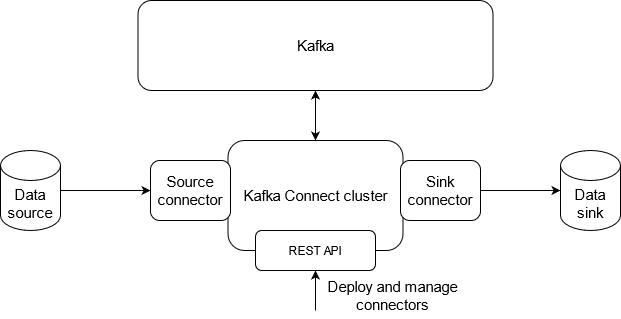
\includegraphics[width=12cm]{images/connector-kafka.png}
	\caption{Kafka Connect cluster to integrate data between Kafka and external data systems.}
	\label{fig:connectkafka}
\end{figure}

Internally, the workers in the connect cluster use Kafka clients to publish or consume data from Kafka. These worker coordinate with each other using the same balancing and failover mechanism as the Kafka consumer group. The framework automatically and periodically checkpoints the current processing positions on the source system of the copying task in Kafka. Developers do not have to take care of managing the consumption status of connector.

For the source connector which imports data into Kafka, the auto-management of consumption status cannot provide exactly-once guarantee in case of failure. This is because the framework does not use transactional feature of Kafka producer to save processing position along with the imported records \cite{kafkaconnectsource}. Therefore, if a worker node crashes before it checkpoints the consumption status on source system to Kafka, it is possible that some records will be reprocessed again when the copying task is resumed. 

With the sink connector which exports data from Kafka, users have the possibility to flush the offset number of the currently consumed record on the Kafka topic along with the actual data in a single atomic action to external data systems. Therefore, when worker node fails, the task can be resumed with the committed offset number on the external system instead of using the checkpointed position on Kafka. As a result, exactly-once semantics can be guaranteed on the sink system. For example, the sink connector to export data from Kafka to HDFS uses this approach to guarantee exactly-once semantics \cite{kafkahdfsconnector}.


With Kafka connector, users can also define a chain of simple and pluggable transformation operations to modify the records one by one before they are written to destination systems \cite{kafkaconnect}. This can serve as a quick preliminary adaption of records so that they can match with the processing logic in their destination.

There are already many off-the-shelf connectors available for various data systems. The Confluent Hub, which is managed by the Confluent company, is a central repository to share Kafka connectors with both open-sourced and commercial licenses. There are connectors of many common data systems such as relational database, Hadoop distributed file system (HDFS), Cassandra, change data capture (CDC) on the source system. All these connectors can be quickly configured and deployed to a Kafka Connect cluster without any implementation. This can further offload the development burden on users to integrate Kafka with other data systems.

\newpage

\textbf{Supported programming languages for clients}\\
The official release of Kafka includes only the Java client \cite{kafkaclients}. Kafka relies on different smaller groups of developers for providing clients in different programming languages. There are many third-party projects with more than 15 different supported programming languages such as C/C++, Python, Go. Most of these projects are very active and regularly updated with each new release from Kafka.  

\large \textbf{Apache Pulsar}\\
\normalsize
\textbf{Connectors to external system}\\
Pulsar supports the automation of moving data in and out of Pulsar with the Pulsar IO connectors \cite{pulsario}. The concept of Pulsar IO is similar to Pulsar Functions. Developers can implement connectors using a Java programming interface provided by Pulsar. 

The executable files of connectors can then be deployed to the cluster of function workers on the Pulsar cluster using the REST API of the cluster or the admin command line tool of Pulsar. The connector is then run and scaled among the nodes of the function workers. 
Internally, Pulsar IO also uses normal Pulsar producer and consumer to interact with the Pulsar cluster. However, unlike the Kafka Connect framework, the management of reading position on the source system is not done transparently to users by Pulsar IO. Developers must handle the task of checkpointing the current consumption status of a connector and retrieving it when the connector is restarted. Therefore, the delivery semantics of a connector depends on the developers and which mechanism they use to commit the reading position. With the newly released Pulsar transaction, developers can utilize this feature to achieve exactly-once semantics for the connector. For instance, transaction is used in the implementation of sink connector to export data from Pulsar to Fink \cite{pulsarflinkconnector}.

In the official release of Pulsar, there are many ready-to-be-used source- and sink-connectors for different data systems such as relational databases, Kafka, HDFS, NoSQL databases. Users can simply start these connectors on the Pulsar cluster without having to download and deploy these connectors manually. There are also many other connectors developed and maintained by third-party organizations. For instance, Streamnative, which is a company offering managed Pulsar as a service, has a central hub with many Pulsar connectors.  

\textbf{Supported programming languages for clients}\\
Officially Apache Pulsar supports 7 different clients in different programming languages including some most popular languages such as Java, Python, and Node.js \cite{pulsarclients}.  Moreover, there are also other clients in 4 different languages all of which are actively maintained by third-party contributors. 

\large \textbf{NATS Streaming}\\
\normalsize
\textbf{Connectors to external system}\\
Currently there is not any general framework to move data in and out of NATS Streaming servers. There are only a few other projects which bridge NATS Streaming with some specific data systems such as Kafka and IBM-MQ \cite{natsclientsconnectors}. Moreover, these off-the-shelf connectors have to be deployed, managed and scaled manually by users. Other than that, if users want to connect NATS Streaming with external data systems, they need to handle the task of implementing, deploying and operating the connectors themselves. Therefore, integrating data with other systems is generally not supported by NATS Streaming. 

\textbf{Supported programming languages for clients}\\
Synadia, which is the company actively develops and maintains the NATS Streaming project, officially supports clients in 7 different programming languages with some common languages: Java, C, Node.js \cite{natsclientsconnectors}. In addition, there are some other clients maintained by the community. Nevertheless, these projects are very inactive and outdated. Therefore, these third-party clients will not be included in the evaluation.      

\section{Monitoring and Management}
\large \textbf{Apache Kafka}\\
\normalsize
\textbf{Technical monitoring}\\
Kafka supports monitoring on both the brokers and clients \cite{kafkamonitoring}. Kafka brokers collect numerous metrics about their current statuses and expose this information to users using Java Management Extension (JMX) \cite{java2006monitoring}. There are many useful metrics such as request rate, memory usage, connection status. Kafka clients and tools such as producer, consumer, Kafka stream processor and connector support monitoring by reporting numerous built-in metrics with JMX such as request rate, response rate from the server, network rate. 

The metrics exposed by JMX can be displayed and monitored using JMX-compliant tools such as jconsole, Prometheus with the JMX exporter. With this monitoring mechanism, Kafka gives users the flexibility to plug in the metrics into different monitoring systems without being tied to a specific tool. 

Apart from relying on the built-in monitoring mechanism of Kafka, there are also many monitoring tools for Kafka health-check developed by third-party organizations which require only minimal setup and can be quickly started \cite{kafkamonitoringtools1}. Each tool has a different license and provides a different set of functionalities. Therefore, users have a wide selection of available tools to match their needs in different cases.

\large \textbf{Apache Pulsar}\\
\normalsize
\textbf{Technical monitoring}\\
Components in a Pulsar cluster expose their monitoring metrics via HTTP ports in Prometheus format \cite{pulsarmetrics}. The Pulsar brokers provide numerous statistics about their current health and statuses such as usage of CPU, memory and network bandwidth, number of currently connected producers and consumers, total throughput. The Zookeeper and BookKeeper shipped together with the Pulsar release also report many metrics on the opened HTTP ports.
These metrics can be directly collected by Prometheus to monitor and create alerts based on the current health of the Pulsar cluster. 

In addition, Pulsar also provides an off-the-shelf and open-source tool named Pulsar-Manager to manage and monitor Pulsar clusters \cite{pulsarmanager}. It is a tool with web UI which can be quickly deployed and connected to a running Pulsar cluster to provide insight into the current status of the cluster. Moreover, users can also dynamically manage and configure the cluster via the UI of the tool such as updating configuration of Pulsar brokers, creating new topics, resetting reading position of consumers.

\large \textbf{NATS Streaming}\\
\normalsize
\textbf{Technical monitoring}\\
To support monitoring, a NATS Streaming server exposes statistics about its current status via an opened HTTP port \cite{natsmonitoring}. The metrics are returned to users in form of JSON. NATS Streaming also provides a Prometheus exporter to convert the metrics from the server monitoring port into Prometheus format to help users display and monitor the server more conveniently. 

The metrics provided by the streaming server via the monitoring endpoints cover mostly information on the high level such as number of currently connected clients, number of channels, total messages received and persisted by the server, current consumption status of subscribers. Users can also keep track of the more low-level information such as memory and CPU usage, message throughput of the underlying NATS server of the streaming server via the same monitoring port \cite{normalnatsconfig}. 

Although the supported metrics of NATS Streaming server do not have a wide coverage as those provided by Apache Kafka or Apache Pulsar, they can still provide a generally good insight into the current status of the streaming server given the simplicity of NATS Streaming compared to the other two platforms.


\section{Scalability} \label{section:scalability}
\large \textbf{Apache Kafka}\\
\normalsize
\textbf{Scalability of storage and computing server}\\
A Kafka broker serves read/write requests from clients as well as persisting the records on its disk. Therefore, the storage and processing layers are closely related and cannot be scaled independently.  

Topic partition is the basis element to achieve scalability on Kafka. Each partition can have one or more replicas, namely, a leader and a number followers for fault-tolerance. Each replica of a partition resides completely on the disk of a broker in the cluster. Read and write requests from client can only be done on the leader of a partition. Therefore, by distributing the leaders of partitions evenly among the brokers, the load on the serving layer can be balanced. Moreover, for each partition, to have even distribution, a different subset of brokers is selected to keep its replicas on their disks. A new broker can always be added to the cluster to scale up the capacity of both processing and persisting. When new partitions are created, their replicas will be automatically assigned to the new broker for load balancing.
\begin{figure}[h]
	\centering
	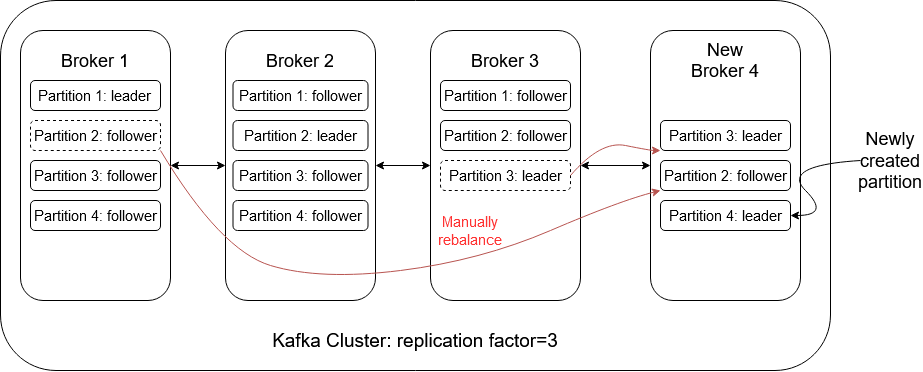
\includegraphics[width=\linewidth]{images/scalability-kafka.png}
	\caption{Kafka clustered is scaled up with a new broker.}
	\label{fig:scalabilitykafka}
\end{figure}

However, for partitions which were created before the new broker is started, their loads are not automatically balanced. In figure \ref{fig:scalabilitykafka}, replicas of partitions 1, 2 and 3 are not automatically offloaded to the new broker. Users must manually conduct the rebalancing using the tools provided by Kafka.

Moreover, the tied coupling between the processing and persisting layers also limits the scalability of Kafka. It could be difficult to optimize the scaling to meets the different requirements on each layer. Therefore, scalability is supported by Kafka. However, the scaling mechanism is quite rigid and requires some manual works from users to rebalance the load. 

\textbf{Broker failover mechanism}\\
In a Kafka cluster, each broker holds the leadership of a subset of partitions and serve requests to these partitions. In case a broker fails, the leadership of each partition will be transferred automatically to one of the brokers retaining the in-sync replica of that partition \cite{kafkadatareplication}. This helps to ensure that the new leader of the partition will have all committed records and guarantee the data consistency. When the failed broker comes back online, by default, users must manually rebalance the leadership again. 

To manage the leadership of partitions among the available brokers, a broker in the cluster is elected as the controller \cite{kafkaleaderelection}. At any time, only one broker can have the role of controller. Currently, Kafka relies on the consistency guarantee of Zookeeper to avoid inconsistent state with more than one active controllers. 

When a broker goes down, the partitions with replicas persisted on the failed broker will become temporarily under-replicated because no auto data re-replication mechanism is provided by Kafka. This may lead to unavailability even when there are still many online brokers as the minimum number in-sync replicas cannot be met. 

\begin{figure}[h]
	\centering
	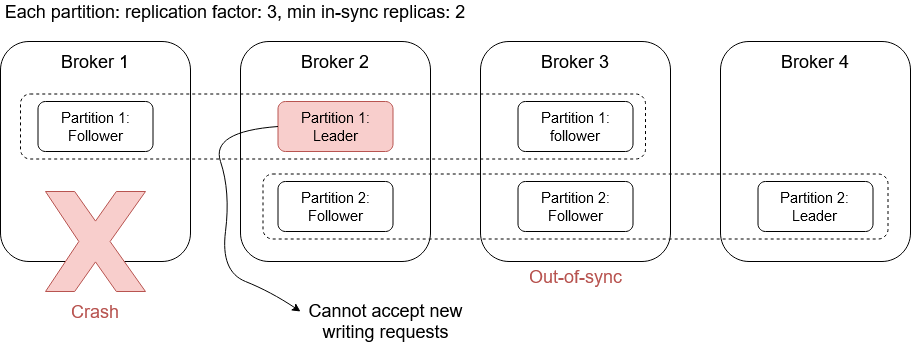
\includegraphics[width=\linewidth]{images/broker-failover-kafka.png}
	\caption{Availability on Kafka cannot be guaranteed when partition is under-replicated.}
	\label{fig:brokerfailoverkafka}
\end{figure}
In figure \ref{fig:brokerfailoverkafka}, when broker 1 fails and the replica of partition 1 on broker 3 becomes out-of-sync with the leader, broker 2 cannot accept new writing requests for partition 1 since it cannot meet the minimum in-sync replicas of two. Broker 4 cannot support to ensure the availability since it does not retain the copy of partition 1. In this case, the availability is compromised for the reliability of data persistence.

If all in-sync replicas including the leader fail at the same time, the remaining replicas of the partition are all lagged behind without having the latest committed messages. In this case, users can choose between availability and consistency of data \cite{kafkadatareplication}. Users can either allow one out-of-sync replica to become the new leader to not disrupt the requests handling and risk losing some records or wait until one in-sync replica goes back online and reject all requests to the failed partition in the meantime. 

Since a Kafka broker also serves the persistence of records, there is a trade-off between its availability and consistency of data. The failover mechanism of Kafka give users the flexibility to manage this trade-off.

\large \textbf{Apache Pulsar}\\
\normalsize
\textbf{Scalability of storage and computing server}\\
In a Pulsar cluster, the cluster of Pulsar brokers is in charge of handling requests from clients while the Bookkeeper cluster is used for data storage. There two layers of processing and storage can be scaled independently.

On the requests-serving layer, each topic is owned by only one broker in the cluster and all requests to this topic will be directed to this broker only. When a new topic is created, the load manager in the Pulsar cluster assigns it to the broker with the least load. Moreover, whenever a broker is overloaded or goes down, the load manager also automatically triggers the balancing to distribute the topics to other brokers \cite{pulsarloadbalance}. As a result, scaling the cluster of brokers is very straightforward. 

On the storage layer, scalability is achieved by the built-in mechanism of Bookkeeper. As elaborated in section \ref{section:eventstorage}, messages are replicated on Bookkeeper cluster in fragments. Each fragment has a different ensemble which is determined by the Pulsar broker. When a new Bookkeeper nodes is started, they will automatically be considered when choosing the ensemble for the next fragment and can start to share the load with other existing nodes. 
\begin{figure}[h]
	\centering
	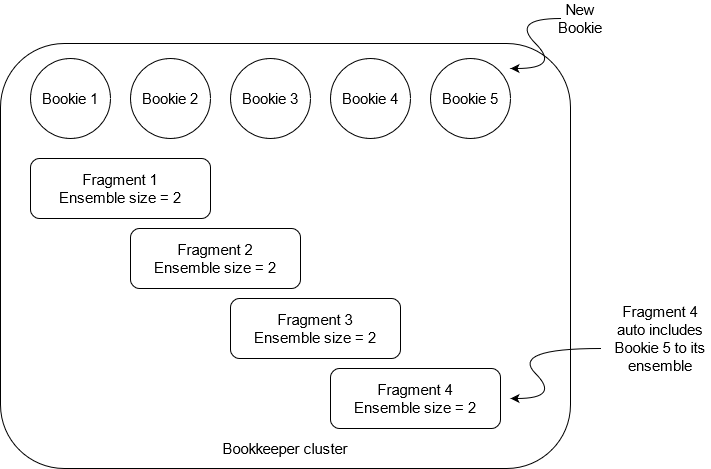
\includegraphics[width=\linewidth]{images/scalability-pulsar.png}
	\caption{Storage layer of Pulsar can be scaled up seamlessly by starting new Bookkeeper instances.}
	\label{fig:scalabilitypulsar}
\end{figure}

If a Bookkeeper node is shut down, some fragments with messages persisted on this node will be under-replicated. However, the auto recovery feature of Bookkeeper can detect this and re-replicate these messages to other running nodes to maintain the replication quorum \cite{bookkeeperadmin}.
\newpage
\textbf{Broker failover mechanism}\\
The brokers are registered to the Zookeeper and regularly kept track of its online status. When a broker is detected to be failed by Zookeeper, its topic will be assigned to other online brokers in the cluster. Apache Pulsar uses the fencing mechanism of BookKeeper to prevent the disconnected broker from writing new message to the topic \cite{bookkeeperprotocol}. This ensures that at any time, only one broker can serve writing requests to a topic.

Because the processing and persisting layers of Pulsar are completely separated, the failover mechanism does not have to consider the reliability of data persistence as in Kafka. As long as there is an online broker, new requests can continue to be accepted. If the requests are handled successfully, clients will receive confirmations from broker and be ensured about the reliability of data. 

\large \textbf{NATS Streaming}\\
\normalsize
\textbf{Scalability of storage and computing server}\\
In both operational modes of NATS Streaming cluster, namely clustering and fault-tolerance, only one server in the cluster can handle read and write requests from clients \cite{natsstreaming}. To support horizontal scaling of requests-serving layer, NATS Streaming provides the partitioning feature \cite{natspartitioning}. This feature is not compatible with clustering mode. With this feature, the normal fault tolerant cluster can be partitioned into a number of smaller sub-clusters, each of which is independently in charge of handling requests for a subset of channels and has a separated datastore to persist messages of these channels. 

Each sub-cluster must be strictly configured with a fixed set of channels. Requests to different channels will be balanced among the server instances in the cluster. New sub-cluster can always be added to the cluster to handle more channels. 
%To save resources with the partitioning feature, active server instance of a sub-cluster can run along with standby instances of other sub-clusters on one host machine. This would not have a significant impact on the performance because the standby instances only forward requests and do not use much resource. 
\begin{figure}[h]
	\centering
	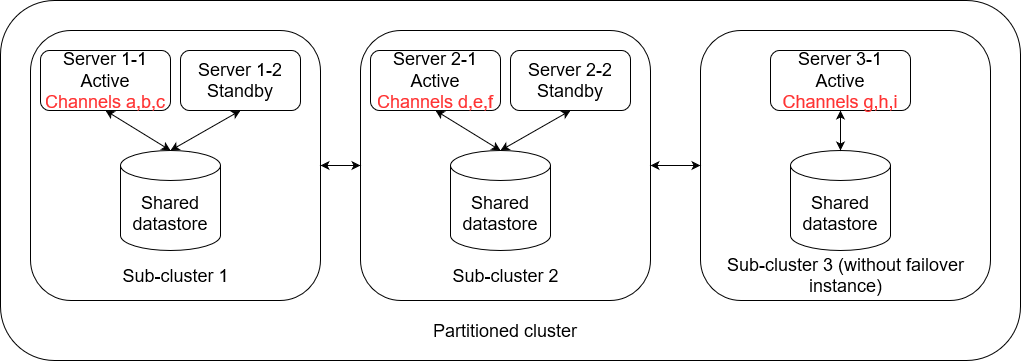
\includegraphics[width=\linewidth]{images/scalability-nats.png}
	\caption{Request-serving layer of NATS Streaming can be scaled with the partitioning feature.}
	\label{fig:scalabilitynats}
\end{figure}

Nevertheless, this scaling mechanism has many limitations. Firstly, this feature cannot be used together with clustering mode. Therefore, it cannot use the data replication feature provided by NATS Streaming. The set of assigned channels for each sub-cluster cannot be changed in runtime. If new channels are required, the sub-cluster must be stopped for reconfiguration. Moreover, because each sub-cluster has a completely separated storage location for all assigned channel, it is not possible to dynamically transfer the ownership of some channels on one sub-cluster to another for load balancing.
 
On the storage layer, the scalability depends on the chosen pluggable data store. For instance, if \emph{file} store is chosen as the persistence layer, a scalable network filesystem can always be used. When \emph{SQL} store is used, the scalability is governed by the relational database technology. However, this relies entirely on the setup of users without any supported feature from NATS Streaming. 

In short, scalability on NATS Streaming is possible for both storage and requests-serving layers. However, most of the configurations and administration tasks are not covered by NATS but instead must be handled manually by users. 

\textbf{Broker failover mechanism}\\
In the clustering mode, the servers in the cluster coordinate with each other using RAFT consensus algorithm \cite{raftalg}. Only the one elected leader in the cluster can serve requests from clients. In case the leader fails, one of the followers will be elected as the new leader. This mode is resilient to split-brain since the Raft algorithm uses majority vote for both leader election and acknowledgement of writing requests. However, if more than half of the servers in the cluster fails, there will be not enough nodes for leader election in case of failure. In this case, the cluster cannot accept new request even when there are still online servers. The availability is automatically compromised for data consistency. 

In the fault-tolerance mode, several server instances are attached to a share datastore \cite{natsstreaming}. At any time, only one active node holds the exclusive lock on the datastore to serve requests. If the active node fails, all standby instances will try to obtain the lock on the data storage and the first to be successful will become the new active node. This failover mechanism requires less overhead as in the clustering mode since no leader re-election is required. In this mode, as long as there is an online server, new requests can be accepted.
\section{Event storage} \label{section:security}
\large \textbf{Apache Kafka}\\
\normalsize
\textbf{Authentication mechanisms}\\
In a Kafka cluster, there are Kafka brokers and Zookeeper nodes. Only legitimate communication peers, namely, reliable Kafka clients, tools which also use Kafka clients internally such as Kafka Connect cluster for data integration and other Kafka brokers in the cluster can initiate connections to a Kafka broker. On the other hand, Zookeeper should be accessed only by Kafka brokers to maintain their metadata. Moreover, Kafka tools also expose REST endpoints for configuration and management such as deploying connectors in case of Kafka Connect. Kafka provides authentication mechanism to control access to all these endpoints \cite{kafkasecurity}.

In order to control access to a Kafka broker, Kafka supports two authentication mechanisms. The first is Transport Layer  Security/Secure Sockets Layer (TLS/SSL) protocol \cite{tls}. Users can configure each communication peer with a valid certificate signed by a mutual trusted Certification Authority (CA) and this will be used for 2-way authentication when establishing the connections between Kafka brokers or between a broker and a client. 

The second mechanism is Simple Authentication and  Security Layer (SASL) \cite{sasl}. Kafka supports 4 different SASL mechanisms out-of-the-box, namely, GSSAPI (Kerberos), PLAIN, SCRAM, and OAUTHBEARER. Users have the flexibility to choose the mechanism which fits to the security system in their existing infrastructures. A broker can also be configured to use multiple authentication mechanisms to support different groups of clients. 

With the Zookeeper soon to be removed from Kafka \cite{kafkaremovezookeeper}, the connection to Zookeeper will also become irrelevant. Nevertheless, in the current release 2.6.0, the connection to Zookeeper must still be protected by either TLS/SSL or SASL. For authentication with SASL, Zookeeper supports two mechanisms: Kerberos and DIGEST-MD5 \cite{zookeepersecurity}. However, the DIGEST-MD5 mechanism is already obsolete and should not be used in production.

Regarding the REST endpoints of the Kafka tools, Kafka supports authentication of connected users with TLS/SSL certificates. 

\textbf{Authorization mechanisms}\\
Kafka allows users to control different level of privilege and a different set of allowed operations for each connected client by providing an Access Control List (ACL) authorizer \cite{kafkasecurity}. This authorizer utilizes the identity of communication peers obtained from the authentication process to determine their access rights. The authorizer supports fine-grained access control for each client with each type of operation on each different resource. Users can define the access right for clients with the general format: \emph{Principal P is [Allowed/Denied] Operation O From Host H on any Resource R matching ResourcePattern RP}. In the current release, the access rights list is persisted by Kafka on Zookeeper. 

However, with the ACL authorizer, users must specify access rights for each and every client individually. Higher level of control, namely, Role-Based Access Control (RBAC) which allows to group multiple clients into one role adhered to only one access rule, is not possible. If this is needed, users must plug in a self-implemented authorizer which can bind the identities to different roles and define different access rules. 

On the other hand, for the connections from Kafka brokers to Zookeeper, Kafka automatically applies the access rules which allow only authenticated brokers to modify metadata stored on Zookeeper. This helps prevent unauthorized modification of metadata which may lead to cluster disruption.

\textbf{Encryption}\\
Kafka only supports encryption when transferring data using TLS/SSL \cite{kafkasecurity}. More specifically, the connections between Kafka brokers and clients, between two brokers, from broker to Zookeeper, and connections to REST endpoints of Kafka tools can be encrypted using the Public-Key Cryptography. Other than that, Kafka supports neither encryption of data at rest nor end-to-end encryption between two end clients.  

\begin{figure}[h]
	\centering
	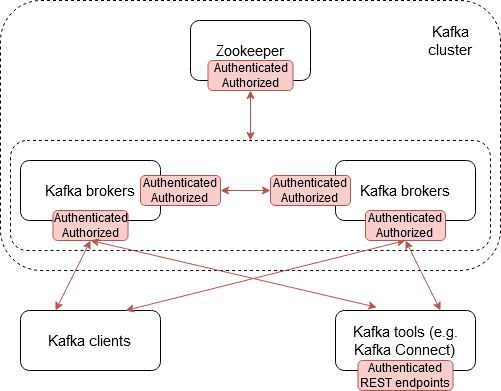
\includegraphics[width=10cm,height=7.5cm]{images/security-kafka.png}
	\caption{Secured Kafka cluster. Red links are encrypted.}
	\label{fig:securitykafka}
\end{figure}

\large \textbf{Apache Pulsar}\\
\normalsize
\textbf{Authentication mechanisms}\\
A Pulsar cluster comprises of multiple components. There are the Pulsar brokers, the Bookkeeper cluster and the Zookeeper nodes. In addition, when Pulsar Function or Pulsar IO is used and configured to be run separately from the brokers, there are also nodes of function workers in the cluster. All these components are interconnected. Pulsar provides different authentication mechanisms to protect these components against unauthorized accesses \cite{pulsarsecurity}.

For the Pulsar brokers and function worker nodes, Pulsar supports different authentication mechanisms. Clients connecting to a broker can be verified using mutual authentication of TLS/SSL protocol \cite{tls}. SASL authentication \cite{sasl} can also be used. Pulsar currently supports two SASL mechanisms which are OAUTHBEARER and GSSAPI (Kerberos). Moreover, with the OAUTHBEARER mechanism, Pulsar also provides a built-in tool to generate and verify token for client identification without having to rely on an additional authorization server. Authentication on Pulsar can also be done with Athenz, which is an open-source platform developed by Yahoo for authentication and authorization based on certificates

A Pulsar broker can be configured with multiple authentications mechanisms. Any client which wants to connect to this broker such as Pulsar producer, consumer, admin client, another broker or function worker must provide its identity with one of the supported authentication schemes of the broker. 

For the connections from Pulsar brokers to Zookeeper and Bookkeeper nodes, they can be protected with either SASL Kerberos authentication mechanism or TLS/SSL certificate-based authentication. Finally, for the connection from Bookkeeper to Zookeeper, users can also configure the authentication using TLS/SSL to control access.

\textbf{Authorization mechanisms}\\
To control access of authenticated clients to resources on Pulsar brokers and function workers, Pulsar provides a built-in authorizer to define ACL \cite{pulsarsecurity}.

The resources provided by Pulsar brokers are hierarchical. At the lowest level is topic from which clients can produce and consume messages. The next level is namespace which is a group of related topics. Then there is tenant resource which is a administrative unit consisting of multiple namespaces. Finally, at the highest level is the cluster. User can grant access to different type of resources on different levels for each authenticated client.

Pulsar does not support RBAC. Currently, there is not any mechanism to define and bind roles to clients and control access based on that.

For resources on Zookeeper and Bookkeeper, it is not documented. Therefore, it can be assumed that Pulsar manages the authorization internally and does not expose the control to users. 

\textbf{Encryption}\\
All connections in a Pulsar cluster can be encrypted with the TLS/SSL protocol. Moreover, Pulsar clients also supports end-to-end encryption \cite{pulsarsecurity}. This is achieved by combining symmetrical encryption and public-key encryption methods. A Pulsar producer can dynamically generate a symmetric key to encrypt payloads of messages. This symmetric key is then encrypted using a different public key in a public-private key pair and included in the header of the messages. On the consumer side, the consumer can use the corresponding private key to decrypt and retrieve the symmetric key used for payload encryption and then use that to read the messages. However, the distribution of the public-private key pair to the clients is not covered by Pulsar. Users must handle this task manually. 

\begin{figure}[h]
	\centering
	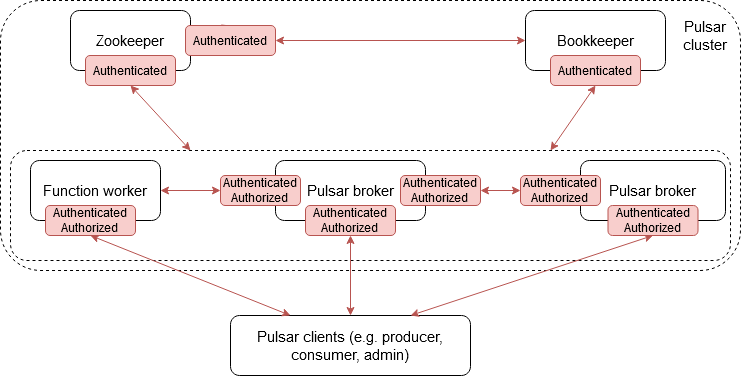
\includegraphics[width=15cm,height=6.5cm]{images/security-pulsar.png}
	\caption{Secured Pulsar cluster. Red links are encrypted.}
	\label{fig:securitypulsar}
\end{figure} 

\large \textbf{NATS Streaming}\\
\normalsize
\textbf{Authentication mechanisms}\\
A NATS Streaming server comprises of a NATS Server and a separated streaming module to provide durability of messages on top of the volatile NATS messaging system. 

NATS Streaming relies on the authentication mechanisms of normal NATS Server to control incoming accesses from clients \cite{normalnatsconfig}. In addition, since the streaming module is also a NATS client internally, it must also use the provided authentication mechanisms to connect to the NATS Server and serve requests from clients. On the other hand, since the durable storage is pluggable, it is beyond the scope of NATS Streaming to provide authentication for this component. Users must utilize the mechanism provided by the selected datastore.

Clients connected to the NATS server can be identified with mutual authentication using TLS/SSL protocol. NATS also provides a number of built-in authentication mechanisms. Users can configure the server and clients with a shared secret which will be used for authentication when a connection is established. NATS also provides a NATS-exclusive authentication mechanism which is public-key based and called NKey. Upon receiving connection request from a client, the server randomly generates a random value and challenges the client to encrypt that with its private key. The server can then verify the response from client by using the public key of the clients. With this authentication mechanism, NATS provides its own tool to generate public-key pairs and verify their legitimacy during authentication.

Nevertheless, apart from the authentication with TLS/SSL, the other authentication mechanisms are only NATS-specific. This lack of support for pluggable and common authentication mechanisms limits the adaptability of NATS Streaming to infrastructures with existing authentication services. In these cases, the security of the NATS system must be configured separately which can cause extra works on administration and maintenance.

\textbf{Authorization mechanisms}\\
The underlying NATS server of the streaming server also provides authorization mechanism to control access of individual clients on the resources \cite{normalnatsconfig}. Nevertheless, this mechanism is not compatible with the NATS Streaming \cite{natsauthorization}. 

More particularly, all subscription requests from clients to streaming channels are internally directed to the streaming module via a single non-persistent NATS channel designated for streaming subscriptions. The authorization mechanisms of NATS can only either block all requests of a client to this internal channel or allow any request to go through. As a result, it is not possible to allow a streaming client to subscribe to only a selective set of channels. 

Therefore, authorization is currently not supported on NATS Streaming. 

\textbf{Encryption}\\
Connections from clients to the NATS streaming server and from streaming module to the NATS server can be encrypted with the TLS/SSL protocol \cite{normalnatsconfig}. The connection from streaming module to the datastore is not covered by NATS. If this connection needs to be encrypted, users must choose the appropriate encryption scheme which is supported by the selected datastore.

Moreover, NATS Streaming also supports encryption of data at rest. The server can be configured with an encryption key and that will be used by the streaming module to encrypt the payload of all messages before persisting them in the durable storage \cite{natstoreencryption}. However, more fine-grained encryption such as different encryption keys for messages from different clients is not possible on NATS Streaming.
\begin{figure}[h]
	\centering
	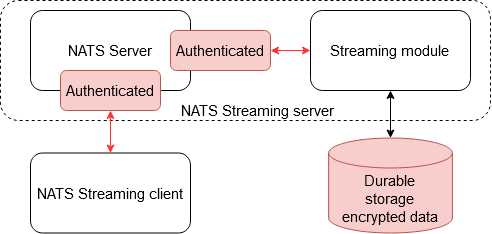
\includegraphics[width=10cm,height=6.5cm]{images/security-nats.png}
	\caption{Secured NATS Streaming cluster. Red links are encrypted.}
	\label{fig:securitynats}
\end{figure}

\section{Usability and Community} \label{section:usability}
\large \textbf{Apache Kafka}\\
\normalsize
\textbf{Active community}\\
The community of Kafka is very active. Since it is created in 2012, the GitHub repository of Kafka has been regularly committed. Starting from the end of 2015, the activity of the community increases significantly with an average of roughly 20 commits per day. In the top 30 contributors, each of them has made more than 50 commits to the project. Many of the contributors are from Confluent which is the company founded by the creators of Kafka. Nevertheless, there are also numerous contributors coming from different organizations and institutions as well.

\begin{figure}[h]
	\centering
	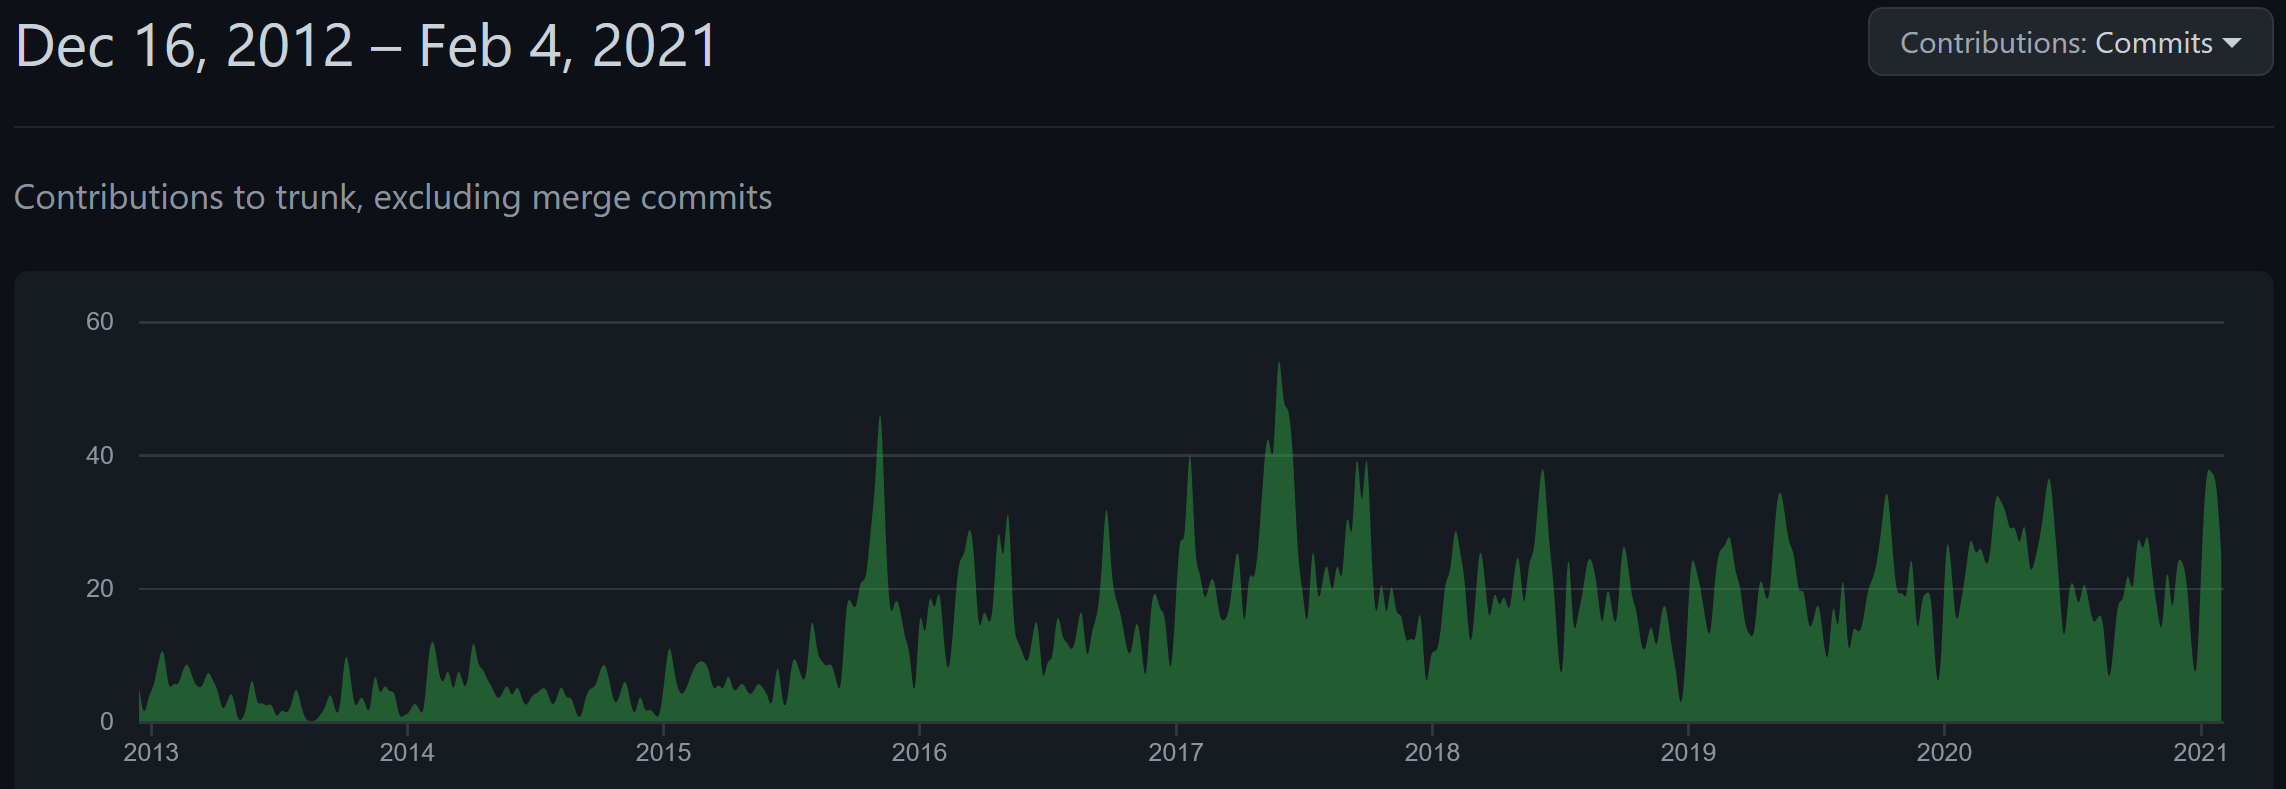
\includegraphics[width=11cm,height=4.5cm]{images/community-kafka.png}
	\caption{Contributions to Kafka on GitHub \cite{kafkarepo}.}
	\label{fig:communitykafka}
\end{figure}

In December 2020, more than 50 contributors made 160 commits to the repository. In this month, there are also around 50 new pull requests and more than 100 merged pull requests on the project.

\large \textbf{Apache Pulsar}\\
\normalsize
\textbf{Active community}\\
\begin{figure}[h]
	\centering
	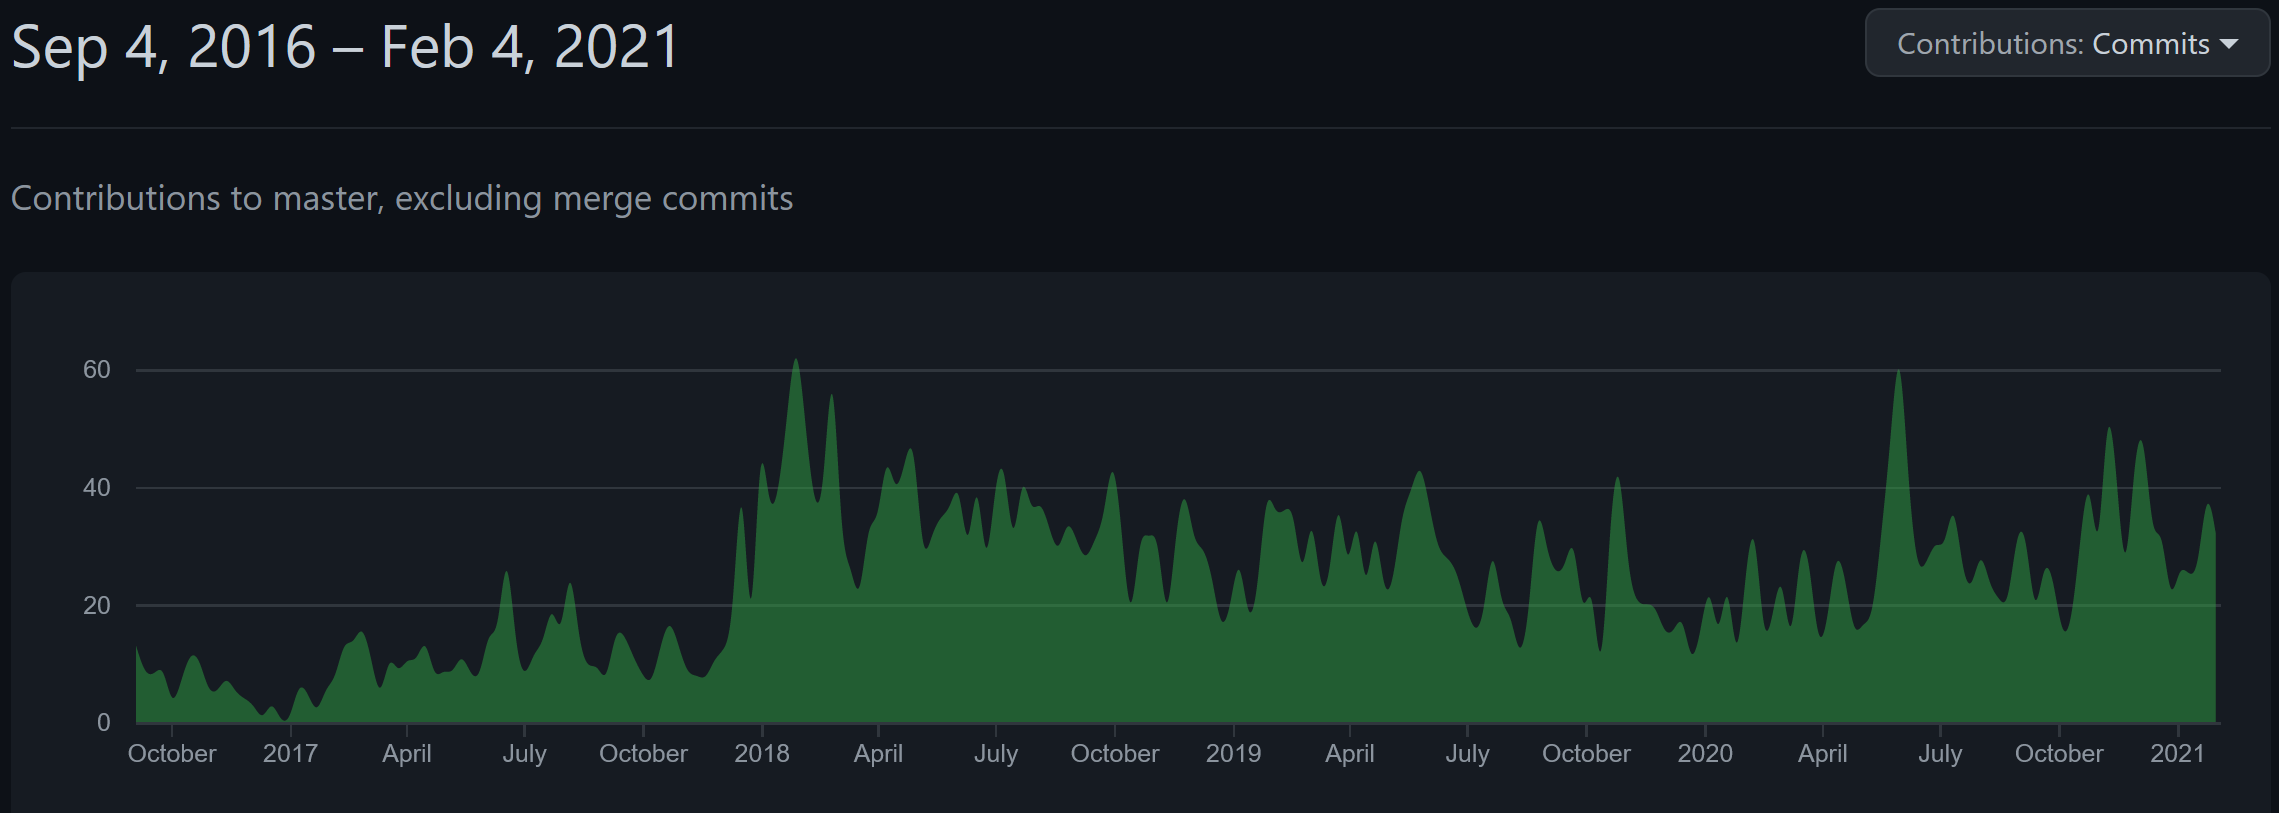
\includegraphics[width=11cm,height=4.5cm]{images/community-pulsar.png}
	\caption{Contributions to Pulsar on GitHub \cite{pulsarrepo}.}
	\label{fig:communitypulsar}
\end{figure}

Since 2016, the Apache Pulsar has been steadily contributed by the community. From 2018, Apache Pulsar has gained more interest from the community with the increase in commits to about 30 commits per day. Each of the top 20 contributors have made more than 50 commits to the project. Many top contributors come from Splunk and Streamnative which are two companies providing managed services based on Apache Pulsar. In addition, there are also many contributors from the different organization actively engaging in the project.

In December 2020, 360 commits have been made by 56 contributors on the Pulsar project. Moreover, more than 200 pull requests are active during this time. 

\large \textbf{NATS Streaming}\\
\normalsize
\textbf{Active community}\\
From the data on GitHub, the NATS Streaming project is not very active, especially since 2018 with an average of around 3 to 4 commits per day. Moreover, only the top 3 contributors have made most of the commits to the project and two of them are from Synadia which is the company creating the NATS system. The other contributors only make minors commit to the project. 

\begin{figure}[h]
	\centering
	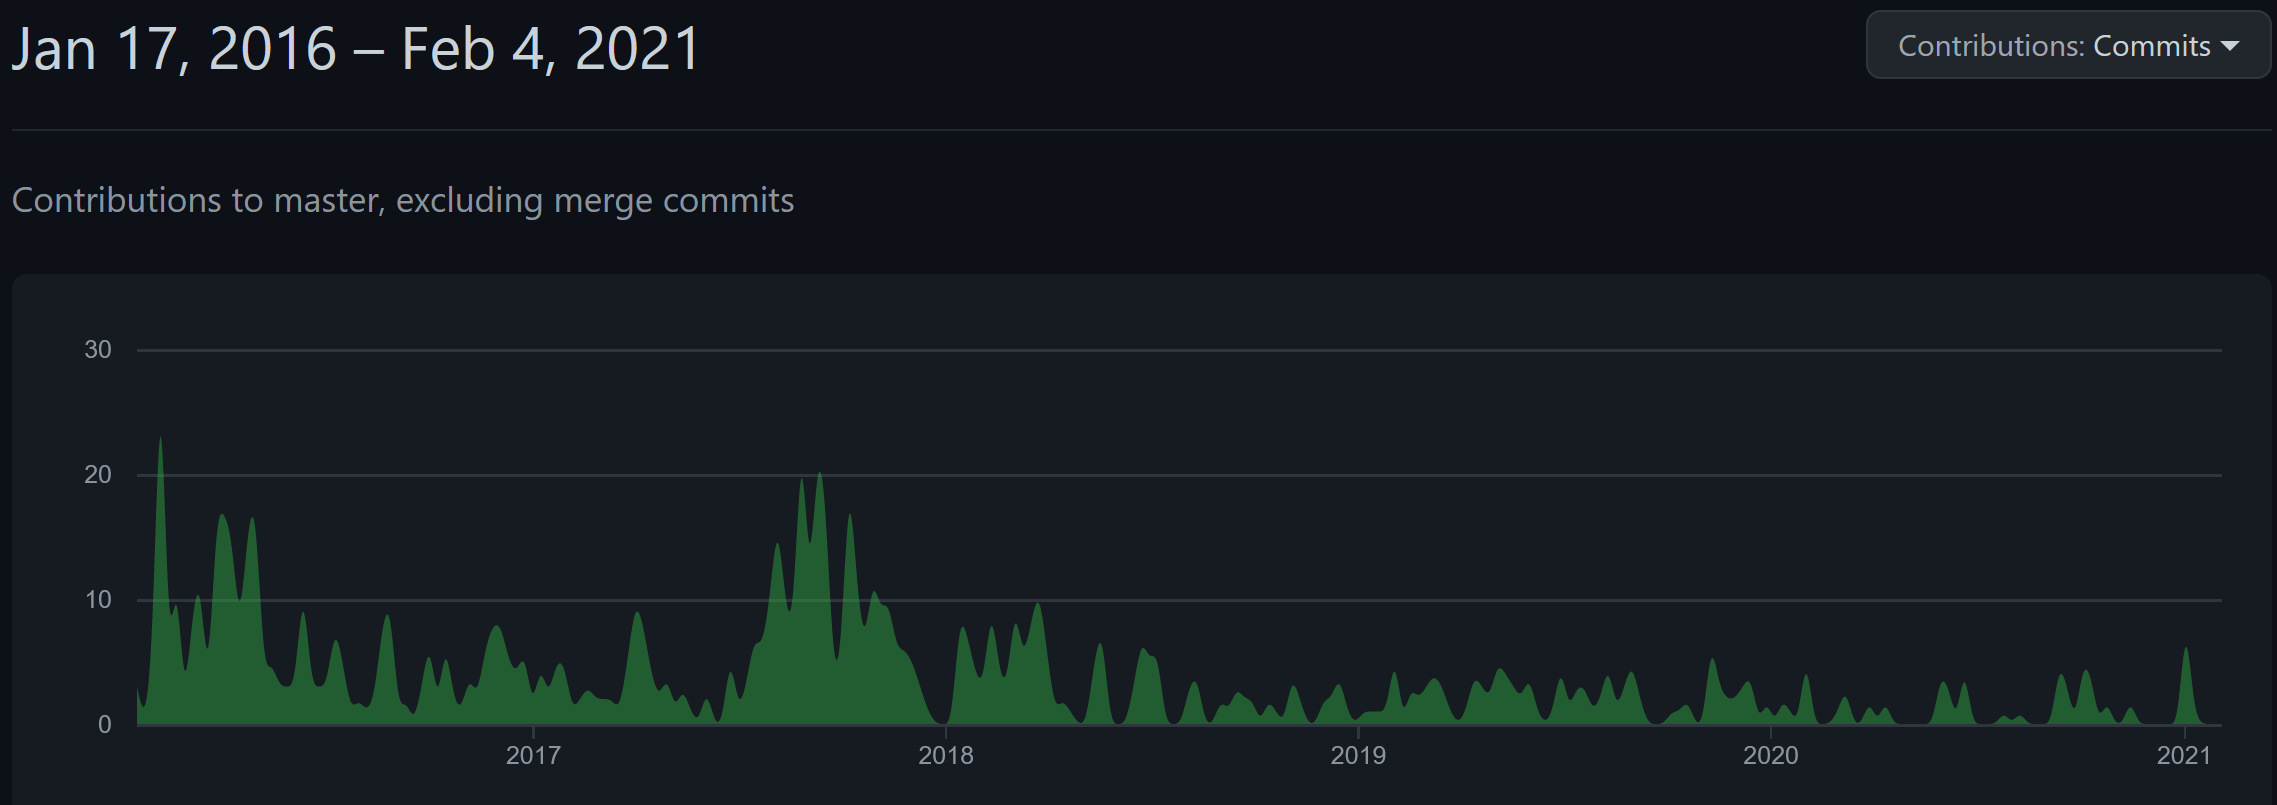
\includegraphics[width=11cm,height=4.5cm]{images/community-nats.png}
	\caption{Contributions to NATS Streaming on GitHub \cite{natsrepo}.}
	\label{fig:communitynats}
\end{figure}

In the month December 2020, no commit has been made on the NATS Streaming repository. In addition, during this month, no pull request is created or merged. 


\section{Performance} \label{section:performance}
There are many comparisons on the time behaviors of most common message delivery systems including Apache Kafka, Apache Pulsar and NATS Streaming. However, the benchmarking results from the comparison of the company SoftwareMill \cite{benchmarkfull} are used in this thesis for the evaluation based on a number of reasons. Moreover, this test takes into consideration all three platforms and provides a uniform benchmark setup for comparison. Finally, since this comparison is done by an independent company, the result can be more objective compared to the benchmarking done by the company Confluent which endorses Kafka \cite{benchmarkkafkapulsarrabbitmq} or the comparison by the StreamNative company which advocates Pulsar \cite{benchmarkkafkapulsar}.

The setup of the test includes a cluster of servers and a number of client instances (producers and consumers) all running on AWS EC2 instances. In the benchmarking, each message is required to have three replicas on different server nodes. Therefore, the cluster of each ESP platform is set up accordingly. 

\underline{Apache Kafka}: Three Kafka brokers running on three different EC2 instances. In addition, there is also a Zookeeper instance running on the same EC2 node with each broker. The replication factor is configured to 3 and the minimum in-sync replica is set to 2.

\underline{Apache Pulsar}: There are three Bookies running on three different EC2 instances. Two Pulsar brokers are started on two different EC2 instances. In addition, there are three separated Zookeeper nodes. The write quorum and acknowledge quorum are set to 3 and 2 respectively.

\underline{NATS Streaming}: Three NATS Streaming server instances are started on three different EC2 instances. The servers are configured to use file store to persist messages on their mounted disks and to run in clustering mode for data replication. 

In the benchmarking scenario, producers and consumers use one topic or channel to send and receive messages. The producers are configured to synchronously wait until the server acknowledge that the published messages are safely persisted and replicated. With Kafka, the producer has to wait for acknowledgment from all in-sync replicas. For Pulsar, On the consumers side, at-least-once delivery guarantee is chosen. The consumers can asynchronously acknowledge the consumption of messages to the server.

The throughput of the messages on both publishing and consuming sides are measured in messages per second with all messages having the same size. The end-to-end latencies of each message within a 1-minute window are also measured and the 95th percentile value is recorded in the result.  

Moreover, in the tests of Apache Pulsar and Apache Kafka, the topic is partitioned to balance the load among the brokers and maximize the utilization of the available processing capability. In the test, the Pulsar topic is only partitioned into 4 because adding more partitions to the topic does not enhance the performance.

\begin{table}[h]
	\centering
	\begin{adjustwidth}{-1cm}{}
	\begin{tabular}{|l|l|l|l|l|l|l|l|}
		\hline
		& Partitions                                              & \begin{tabular}[c]{@{}l@{}}Threads\\ /node\end{tabular} & \begin{tabular}[c]{@{}l@{}}Sender \\ nodes\end{tabular} & \begin{tabular}[c]{@{}l@{}}Receiver\\ nodes\end{tabular} & \begin{tabular}[c]{@{}l@{}}Producing\\ throughput\\ (msgs/s)\end{tabular} & \begin{tabular}[c]{@{}l@{}}Consuming\\ throughput\\ (msgs/s)\end{tabular} & \begin{tabular}[c]{@{}l@{}}End-to-end\\ latency\\ (ms)\end{tabular} \\ \hline
		\begin{tabular}[c]{@{}l@{}}Apache\\ Kafka\end{tabular}   & 64                                                       & 25                                                      & 8                                                       & 16                                                       & 272 828                                                                    & 272 705                                                                    & 48                                                                  \\ \hline
		\begin{tabular}[c]{@{}l@{}}Apache\\ Pulsar\end{tabular}  & 4                                                        & 25                                                      & 8                                                       & 16                                                       & 176 439                                                                    & 176 388                                                                    & 50                                                                  \\ \hline
		\begin{tabular}[c]{@{}l@{}}NATS\\ Streaming\end{tabular} & \begin{tabular}[c]{@{}l@{}}Not\\ applicable\end{tabular} & 25                                                      & 8                                                       & 16                                                       & 26 699                                                                     & 26 696                                                                     & 148                                                                 \\ \hline
	\end{tabular}
 \end{adjustwidth}
 \caption{Benchmarking results of Kafka, Pulsar and NATS Streaming \cite{benchmarkfull}.}
\label{table:performance}
\end{table}
\iffalse
\begin{table}[h]
	\centering
	\caption{Benchmarking results of Kafka, Pulsar and NATS Streaming.}
	\label{table:performance}

	\begin{tabular}{|l|l|l|l|l|l|l|l|}
		\hline
		& Partitions     & Threads/node & Sender nodes & Receiver nodes & Producing throughput (msgs/s) & Consuming throughput (msgs/s) & End-to-end latency (ms) \\ \hline
		Apache Kafka   & 64             & 25           & 8            & 16             & 272 828                       & 272 705                       & 48                      \\ \hline
		Apache Pulsar  & 4              & 25           & 8            & 16             & 176 439                       & 176 388                       & 50                      \\ \hline
		NATS Streaming & Not applicable & 25           & 8            & 16             & 26 699                        & 26 696                        & 148                     \\ \hline
	\end{tabular}

\end{table}
\fi
With the same number of sending and receiving threads, Apache Kafka is outstanding with the throughput of approximately 270 000 messages per second and the 95th percentile value of latency around 48 milliseconds. Next is Apache Pulsar with the throughput of roughly 170 000 messages per second. The end-to-end latency of Pulsar is as good as Kafka with 50 milliseconds. NATS Streaming performance is not as good as the other platforms with throughput of only 26 000 messages per second and latency of 148 milliseconds. This is understandable since only one server instance in the NATS cluster can serve requests. 

To summary, with the same hardware capacity, Kafka has the best performance in term of both throughput and end-to-end latency. Apache Pulsar comes in the middle with the same latency as Kafka and lower throughout. NATS Streaming has the lowest throughput and the highest end-to-end latency. Since Kafka is leading among three platforms, its performance will be used as the standard benchmark for grading in the final feature matrix. 

\section{Feature matrix} 
Finally, the evaluation results of three platforms are put together and incorporated into the feature matrix. The general structure of the matrix is showed in figure \ref{fig:featurematrix}.

\begin{figure}[h]
	\begin{adjustwidth}{-1.5cm}{}
	\centering
	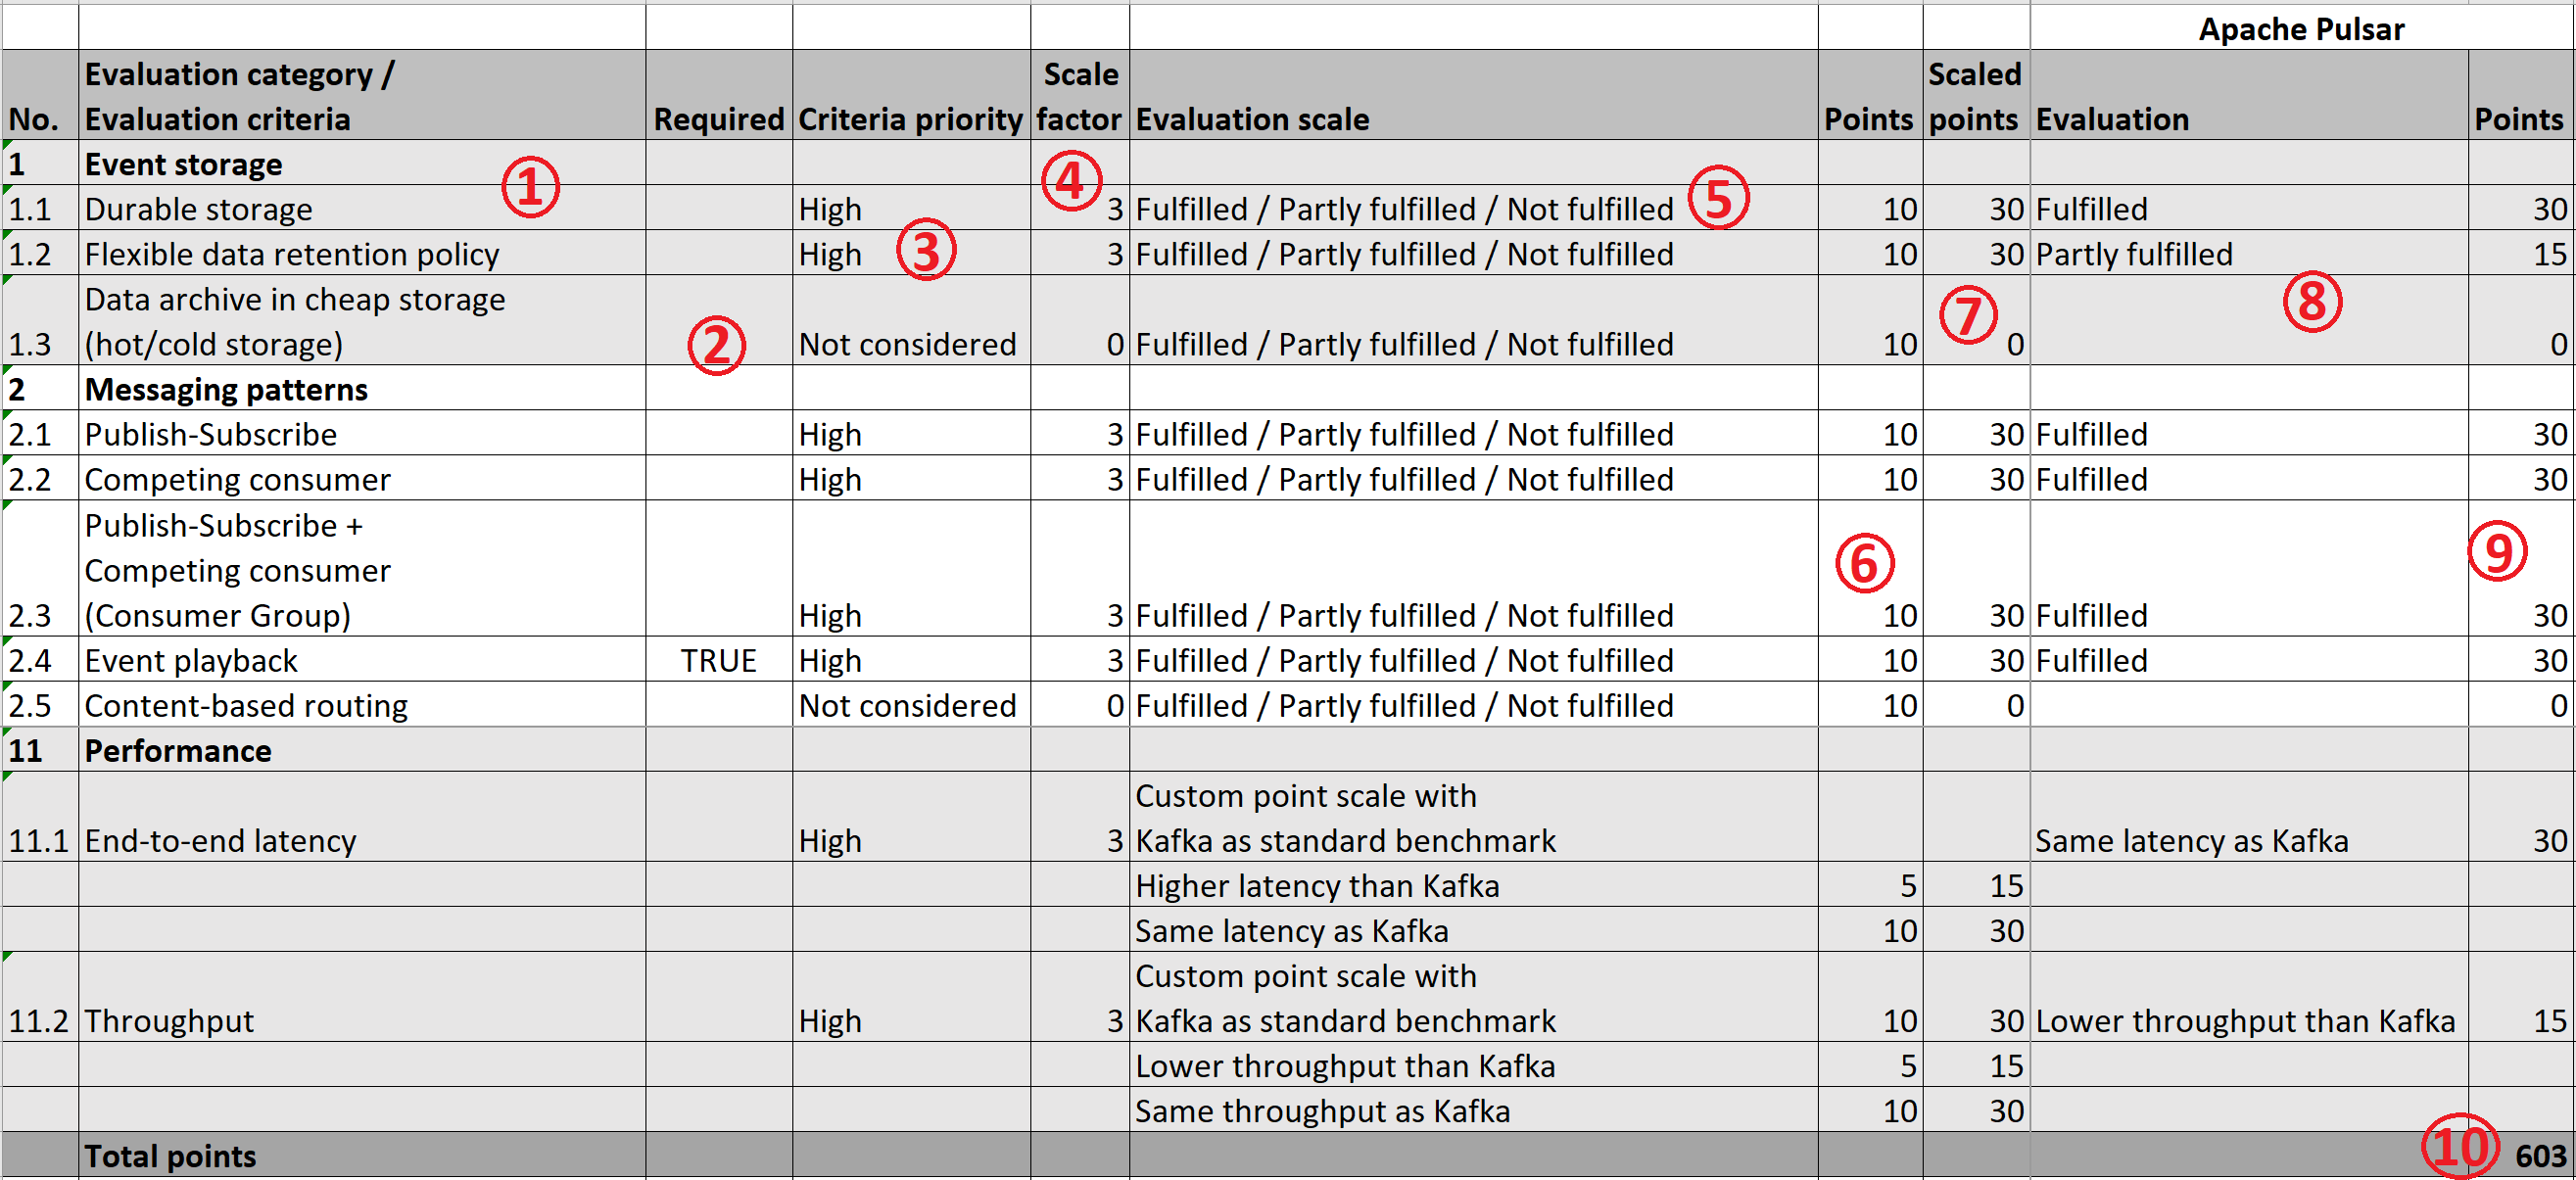
\includegraphics[width=18cm,height=4.5cm]{images/feature-matrix.png}
	\end{adjustwidth}
	\caption{General structure of the feature matrix.}
	\label{fig:featurematrix}
\end{figure}

In the matrix, users has the flexibility to choose different priority for each criterion. 